%================= PREAMBULE =================
\documentclass[12pt,a4paper]{report}

\usepackage[utf8]{inputenc}
\usepackage[T1]{fontenc}
\usepackage[french]{babel}
\usepackage{lmodern}
\usepackage{amsmath,amssymb,amsthm}
\usepackage{geometry}
\geometry{margin=2.5cm}
\usepackage{tabularx}
\usepackage[dvipsnames,table]{xcolor}
\usepackage{ragged2e}
\usepackage{grffile}
\usepackage{booktabs}
\usepackage{longtable}
\usepackage{multirow}
\usepackage{colortbl}
\usepackage{hhline}
\usepackage{calc}
\usepackage{subcaption}
\usepackage{wrapfig}
\usepackage{microtype}
\usepackage{emptypage}
\usepackage{caption}

\usepackage{setspace}
\onehalfspacing
\usepackage{graphicx}
\usepackage{float}
\usepackage{array,booktabs}

% Couleurs & style des titres
\usepackage{xcolor}
\definecolor{myblue}{RGB}{0,51,153} % bleu foncé
\definecolor{capgeminiblue}{RGB}{0,112,184}
\definecolor{lightgray}{RGB}{245,245,245}
\definecolor{darkgray}{RGB}{64,64,64}
\usepackage{sectsty}
\sectionfont{\color{myblue}}
\subsectionfont{\color{black}}
\subsubsectionfont{\color{black}}

% Configuration des légendes
\captionsetup{
    format=hang,
    font={small,bf},
    labelfont={color=capgeminiblue,bf},
    margin=1cm,
    skip=20pt,
    position=bottom,
    justification=centering
}

% Hyperliens (après xcolor)
\usepackage{hyperref}
\hypersetup{
  colorlinks=true,
  linkcolor=black,
  urlcolor=myblue,
  citecolor=myblue
}

% Pied de page
\usepackage{fancyhdr}
\pagestyle{fancy}
\fancyhf{}
\fancyfoot[C]{\thepage}
\renewcommand{\headrulewidth}{0pt}

% Ajustement pour headheight
\setlength{\headheight}{25pt}

\begin{document}
\thispagestyle{empty} % Supprime le numéro de page

\begin{center}

% Logos en haut
\begin{minipage}{0.45\textwidth}\centering
  
\includegraphics[height=6.5cm]{latex_media/media/image1.png}
\end{minipage}\hfill
\begin{minipage}{0.45\textwidth}\centering
  
\includegraphics[height=3.5cm]{latex_media/media/image3.png}
\end{minipage}

\vspace{1cm}

{\Large \textbf{PROJET DE FIN D'ÉTUDES}}\\[0.5cm]

{\Large \textbf{Développement d'une application de gestion de quiz \\
pour l'évaluation des compétences en agilité}}\\[1cm]

{\large Filière: \textbf{Ingénierie Informatique et Réseaux (5\ieme{} année)}}\\[1.2cm]


\includegraphics[height=3cm]{latex_media/media/image3.png}\\[0.4cm]

{\large \textbf{Organisme d'accueil: CAPGEMINI}}\\[1.5cm]

\begin{tabular}{@{}>{\bfseries}r l@{}}
  Réalisé par:& ANIBA SOUFIANE \\
  Encadrant(s) professionnel(s):& [NOM ENCADRANT] \\
  Encadrant pédagogique:& [NOM ENCADRANT] \\
\end{tabular}

\vfill
{\large Année universitaire: \textbf{2024/2025}}

\end{center}

% ---------------- Dédicaces (nouvelle page) ----------------
\clearpage
\thispagestyle{empty}
\begin{center}
    {\Large\bfseries Dédicaces}\par
    \vspace{1.2cm}

    \begin{minipage}{0.85\linewidth}
    \centering
    Je dédie ce travail, fruit de plusieurs mois d'efforts, de recherches et d'engagement,\par
    \vspace{0.6em}

    \textbf{À mes chers parents,}\par
    pour leur amour infini, leurs sacrifices, leurs prières et leur soutien indéfectible
    dans chaque étape de ma vie. Vous êtes ma plus grande source d'inspiration et de force.\par
    \vspace{0.8em}

    \textbf{À mes frères et sœurs,}\par
    pour leur affection, leur complicité et leurs encouragements constants,
    qui m'ont soutenu dans les moments les plus exigeants.\par
    \vspace{0.8em}

    \textbf{À mes grands-parents et à toute ma famille,}\par
    pour leur bienveillance, leurs prières et leur confiance en moi.\par
    \vspace{0.8em}

    \textbf{À mes amis,}\par
    pour leur présence précieuse, leur joie et leurs encouragements qui ont rendu
    ce parcours plus humain et plus agréable.\par
    \vspace{0.8em}

    \textbf{Enfin,}\par
    à toutes celles et ceux qui, de près ou de loin, ont cru en moi,
    m'ont soutenu et motivé tout au long de ce chemin.\par
    \vspace{1.2em}

    \emph{Merci à vous tous.}
    \end{minipage}
\end{center}

\clearpage

%================= PAGE 3 — REMERCIEMENTS ===============
\cleardoublepage
\pagenumbering{roman} % Commence la numérotation en chiffres romains
\setcounter{page}{1}
\addcontentsline{toc}{chapter}{Remerciements}
\vspace*{1.5cm}

\begin{center}
    {\Large\bfseries Remerciements}\par
    \vspace{1.2cm}

    \begin{minipage}{0.85\linewidth}
    \centering
    J'exprime ma profonde reconnaissance à mon encadrant professionnel chez \textbf{Capgemini}, pour la confiance qu'il m'a accordée, ses conseils avisés et son accompagnement tout au long de cette expérience.\par
    \vspace{0.8em}

    Mes sincères remerciements vont également à \textbf{toute l'équipe} pour son aide précieuse, sa disponibilité et son soutien constant dans la réalisation de ce projet.\par
    \vspace{0.8em}

    Je tiens à remercier chaleureusement \textbf{toute l'équipe technique de Capgemini}, pour leur accueil, leur disponibilité et leur bienveillance, qui ont largement contribué à rendre ce stage formateur et agréable.\par
    \vspace{0.8em}

    Je souhaite également remercier mon encadrant pédagogique pour son suivi rigoureux, ses conseils précieux et son accompagnement tout au long de ces six mois.\par
    \vspace{0.8em}

    Enfin, j'exprime ma gratitude à l'\textbf{École Marocaine des Sciences de l'Ingénieur (EMSI)} pour la qualité de l'enseignement reçu durant ces cinq années de formation, qui m'ont permis de mener à bien ce projet.\par

    \vspace{1.2em}
    \emph{À toutes celles et ceux qui, de près ou de loin, ont contribué à cette réussite: merci infiniment.}
    \end{minipage}
\end{center}
\clearpage

%================= PAGE RÉSUMÉ =================
\cleardoublepage
\addcontentsline{toc}{chapter}{Résumé}
\chapter*{Résumé}

Le présent rapport est l'aboutissement du travail effectué dans le cadre du projet de fin d'études au sein de \textbf{Capgemini} pour l'obtention du diplôme d'Ingénieur en Informatique. L'objectif principal du projet consiste en la conception et le développement d'une application de gestion de quiz pour l'évaluation des compétences en agilité des collaborateurs.

Dans un monde où l'apprentissage continu est essentiel, \textbf{QUIZ AGILE} permet aux entreprises d'évaluer et de suivre les compétences de leurs collaborateurs. Intégrée à la plateforme de formation \textbf{NEXT}, cette solution facilite l'auto-évaluation, personnalise les parcours de formation et offre des analyses précises aux managers.

L'évaluation des compétences en agilité représente un défi majeur pour les entreprises modernes. Les méthodes traditionnelles sont souvent chronophages, subjectives et difficiles à standardiser. \textbf{QUIZ AGILE} répond à cette problématique en proposant une plateforme flexible et évolutive, permettant la création et la gestion de questions de type QCM, la génération de quiz personnalisés, et l'analyse détaillée des résultats.

Durant le déroulement du projet, nous avons commencé par une analyse fonctionnelle et technique des spécifications afin de bien saisir la problématique, puis nous avons entamé l'étape de conception pour finir avec la mise en œuvre. L'application a été développée avec une stack technique moderne comprenant React pour le frontend et Spring Boot pour le backend, avec une approche DevOps intégrant GitLab, Jenkins et Docker.

Pour la mise en place du projet \textbf{QUIZ AGILE}, et pour assurer l'agilité, le choix est tombé sur Scrum comme méthodologie de gestion de projet, avec un cycle de développement itératif et incrémental. Cette approche nous a permis de livrer régulièrement des fonctionnalités à valeur ajoutée et d'adapter le développement aux retours des utilisateurs.

\textbf{Mots clés} : Gestion de quiz, évaluation des compétences, agilité, formation continue, Spring Boot, React, analyse fonctionnelle, conception, mise en œuvre, Scrum.

%================= PAGE ABSTRACT =================
\cleardoublepage
\addcontentsline{toc}{chapter}{Abstract}
\chapter*{Abstract}

This report is the result of the work carried out as part of the end-of-study project at Capgemini, aiming to obtain the Engineering degree in Computer Science. The main objective of the project is the design and development of a quiz management application for assessing employees' agility-related skills.

In a world where continuous learning is essential, \textbf{QUIZ AGILE} enables companies to evaluate and monitor the competencies of their employees. Integrated with the \textbf{NEXT} training platform, this solution facilitates self-assessment, personalizes learning paths, and provides managers with accurate performance analytics.

Assessing agility skills is a major challenge for modern companies. Traditional methods are often time-consuming, subjective, and difficult to standardize. QUIZ AGILE addresses this issue by offering a flexible and scalable platform that allows the creation and management of multiple-choice questions (MCQs), the generation of personalized quizzes, and the detailed analysis of results.

Throughout the project, we began with a functional and technical analysis of the specifications to fully understand the problem. Then, we moved on to the design phase and finally to the implementation. The application was developed using a modern technical stack including \textbf{React} for the frontend and \textbf{Spring Boot} for the backend, following a \textbf{DevOps} approach integrating \textbf{GitLab}, \textbf{Jenkins}, and \textbf{Docker}.

To ensure agility in the development process, the \textbf{Scrum} methodology was adopted, enabling an iterative and incremental development cycle. This approach allowed us to deliver value-added features regularly and to adapt development based on user feedback.

\textbf{Keywords}: Quiz management, skills assessment, agility, continuous training, Spring Boot, React, functional analysis, design, implementation, Scrum

%================= LISTE DES ABRÉVIATIONS ==================
\cleardoublepage
\addcontentsline{toc}{chapter}{Liste des Abréviations}
\chapter*{Liste des Abréviations}

\begin{longtable}[]{@{}
  >{\raggedright\arraybackslash}p{(\columnwidth - 2\tabcolsep) * \real{0.25}}
  >{\raggedright\arraybackslash}p{(\columnwidth - 2\tabcolsep) * \real{0.75}}@{}}
\toprule
\rowcolor{capgeminiblue}
\textcolor{white}{\textbf{Abréviation}} & \textcolor{white}{\textbf{Signification}} \\
\midrule
\endhead
\rowcolor{lightgray}
AJAX & Asynchronous JavaScript and XML (JavaScript et XML Asynchrones) \\
API & Application Programming Interface (Interface de Programmation d'Application) \\
\rowcolor{lightgray}
CI/CD & Continuous Integration/Continuous Deployment (Intégration/Déploiement Continu) \\
CRUD & Create, Read, Update et Delete (Créer, Lire, Modifier, Supprimer) \\
\rowcolor{lightgray}
CSS & Cascading Style Sheets (Feuilles de Style en Cascade) \\
DAO & Data Access Object (Objet d'Accès aux Données) \\
\rowcolor{lightgray}
DOM & Document Object Model \\
DTO & Data Transfer Object (Objet de Transfert de Données) \\
\rowcolor{lightgray}
HTML & HyperText Markup Language (Langage de Balisage HyperTexte) \\
HTTP & HyperText Transfer Protocol \\
\rowcolor{lightgray}
IDE & Integrated Development Environment (Environnement de Développement Intégré) \\
Java & Plateforme de développement orientée objet \\
\rowcolor{lightgray}
JDBC & Java Database Connectivity (Connectivité Base de Données Java) \\
JPA & Java Persistence API (API de Persistance Java) \\
\rowcolor{lightgray}
JSON & JavaScript Object Notation (Notation d'Objet JavaScript) \\
JWT & JSON Web Token \\
\rowcolor{lightgray}
JVM & Java Virtual Machine \\
MVC & Model View Controller (Modèle Vue Contrôleur) \\
\rowcolor{lightgray}
NPM & Node Package Manager \\
ORM & Object-Relational Mapping (Mappage Objet-Relationnel) \\
\rowcolor{lightgray}
QCM & Questionnaire à Choix Multiples \\
RBAC & Role-Based Access Control \\
\rowcolor{lightgray}
REST & Representational State Transfer (Transfert d'État Représentationnel) \\
RGPD & Règlement Général sur la Protection des Données \\
\rowcolor{lightgray}
SCRUM & Méthodologie de gestion de projet agile \\
SDLC & Software Development Life Cycle \\
\rowcolor{lightgray}
SGBDR & Système de gestion de bases de données relationnelles \\
SOLID & Principes de conception orientée objet \\
\rowcolor{lightgray}
SPA & Single Page Application \\
SQL & Structured Query Language (Langage de Requête Structuré) \\
\rowcolor{lightgray}
UI/UX & User Interface/User Experience (Interface/Expérience Utilisateur) \\
UML & Unified Modeling Language (Langage de Modélisation Unifié) \\
\rowcolor{lightgray}
URL & Uniform Resource Locator \\
\bottomrule
\end{longtable}

\begin{center}
\textit{Tableau 1~: Liste des principales abréviations utilisées dans ce rapport}
\end{center}
\cleardoublepage

%================= SOMMAIRE & LISTES ==================
\tableofcontents
\cleardoublepage
\addcontentsline{toc}{chapter}{Liste des figures}
\listoffigures
\cleardoublepage

%================= INTRODUCTION GENERALE =================
\pagenumbering{arabic}
\setcounter{page}{1}
\chapter*{Introduction générale}
\addcontentsline{toc}{chapter}{Introduction générale}

\noindent
Dans un contexte professionnel en constante évolution, les entreprises
font face à un défi majeur : assurer le développement continu des
compétences de leurs collaborateurs. L'agilité, en
particulier, s'est imposée comme une compétence
fondamentale dans le secteur informatique, transformant profondément les
méthodes de travail et la gestion de projets. Cette approche, qui
privilégie l'adaptabilité, la collaboration et
l'amélioration continue, nécessite une maîtrise précise
de concepts et de pratiques spécifiques.

\medskip
\noindent
Cependant, l'évaluation des compétences en agilité
demeure un exercice complexe. Les méthodes traditionnelles
d'évaluation présentent plusieurs limitations : elles
sont souvent chronophages, subjectives, difficiles à standardiser à
l'échelle d'une organisation et ne
permettent pas toujours d'identifier avec précision les
lacunes à combler. De plus, la collecte et l'analyse des
résultats peuvent s'avérer fastidieuses, limitant ainsi
la capacité des entreprises à adapter rapidement leurs parcours de
formation aux besoins réels de leurs collaborateurs.

\medskip
\noindent
Face à ces enjeux, \textbf{Capgemini} a identifié le besoin de
développer une solution innovante permettant d'évaluer
et de suivre efficacement les compétences en agilité de ses
collaborateurs. C'est dans ce cadre que
s'inscrit le projet \textbf{QUIZ AGILE}, une application
de gestion de quiz conçue pour standardiser l'évaluation
des compétences, faciliter l'analyse des résultats et
optimiser les parcours de formation.

\medskip
\noindent
\textbf{QUIZ AGILE} vise à répondre à plusieurs objectifs stratégiques :

\begin{itemize}
    \item Standardiser l'évaluation des compétences en agilité au sein de l'entreprise
    \item Adapter les formations selon les besoins spécifiques identifiés
    \item Favoriser l'auto-apprentissage des collaborateurs
    \item Fournir aux managers des tableaux de bord détaillés sur les compétences de leurs équipes
    \item Créer une base de connaissances évolutive pouvant s'étendre à d'autres domaines de compétences
\end{itemize}

\medskip
\noindent
Pour atteindre ces objectifs, l'application propose un
ensemble de fonctionnalités clés : création et gestion de questions de
type QCM, génération de quiz personnalisés, diffusion via des URL
uniques, analyse détaillée des résultats, et intégration avec la
plateforme de formation NEXT existante. Cette intégration est
particulièrement importante car elle permet de créer un écosystème
complet allant de l'évaluation des compétences à la
formation ciblée.

\medskip
\noindent
Ce mémoire retrace l'ensemble des étapes de ce projet. Il est structuré de la manière suivante:
\begin{itemize}
    \item \textbf{Chapitre I:} Présente le contexte général du projet, l'organisation d'accueil Capgemini ainsi que les objectifs poursuivis.
    \item \textbf{Chapitre II:} Détaille l'étude préliminaire, l'analyse des besoins fonctionnels et non-fonctionnels.
    \item \textbf{Chapitre III:} Expose l'analyse fonctionnelle et conceptuelle, avec les cas d'utilisation et la conception du système.
    \item \textbf{Chapitre IV:} Présente l'étude technique, les choix d'architecture, l'environnement de développement et les outils utilisés.
    \item \textbf{Chapitre V:} Illustre la mise en œuvre concrète du système avec les interfaces clés de l'application.
\end{itemize}

%================= CHAPITRE 1 — PAGE D'OUVERTURE =========
\cleardoublepage
\thispagestyle{empty}
\begin{center}
    \vspace*{4cm}
    {\Huge \textbf{Chapitre 1}}\\[1.5cm]
    {\LARGE \textbf{Contexte Général du projet}}
\end{center}
\cleardoublepage

%================= CHAPITRE 1 — CONTENU ==================
\refstepcounter{chapter}
\addcontentsline{toc}{chapter}{Chapitre \thechapter: Contexte Général du projet}
\markboth{Chapitre \thechapter: Contexte Général du projet}{}
\setcounter{section}{0}

\section{Introduction}

Ce chapitre a pour objectif de présenter le cadre dans lequel notre
projet de fin d'études a été effectué. Nous y trouverons
des détails concernant l'entreprise
d'accueil, son organisation ainsi que ses activités.

Dans la deuxième partie, nous introduirons le projet \textbf{Quiz Agile}
en décrivant brièvement sa raison d'être et ses
objectifs. Cette mise en contexte permettra de mieux comprendre les
enjeux et les défis auxquels le projet répond, ainsi que son importance
stratégique pour \textbf{Capgemini}.

\section{Présentation de l'organisme d'accueil}

\subsection{Groupe Capgemini}

\begin{figure}[htbp]
    \centering
    
\includegraphics[width=0.7\textwidth]{latex_media/media/image3.png}
    \caption{Logo Capgemini}
    \label{fig:logo-capgemini}
\end{figure}

\textbf{Capgemini} est un leader mondial des services de conseil, de transformation numérique, de technologie et d'ingénierie. Le Groupe est à la pointe de l'innovation pour répondre à l'ensemble des opportunités des clients dans le monde en évolution du cloud, du numérique et des plateformes. Le premier en France et le 6ème à l'échelle mondiale conduisant une stratégie de développement et de diversification qui a donné naissance à une croissance interne et externe. \textbf{Capgemini} est responsable de
325 000 personnes dans près de 50 pays. Partenaire stratégique des
entreprises pour la transformation de leurs activités en tirant profit
de toute la puissance de la technologie, le Groupe est guidé au
quotidien par sa raison d'être ; libérer les énergies humaines par la
technologie pour un avenir inclusif et durable. Fort de plus de 55 ans
d'expérience et d'une grande expertise des différents secteurs
d'activité, \textbf{Capgemini} est reconnu par ses clients pour répondre
à l'ensemble de leurs besoins, de la stratégie et du design jusqu'au
management des opérations, en tirant parti des innovations dans les
domaines en perpétuelle évolution du cloud, de la data, de
l'Intelligence Artificielle, de la connectivité, des logiciels, de
l'ingénierie digitale et des plateformes. Le Groupe a réalisé un chiffre
d'affaires de 17 milliards d'euros en 2022.

\subsection{Historique du groupe Capgemini}

L'entreprise \textbf{Capgemini} a été créée en 1967 à Grenoble sous le
nom de Sogeti par Serge Kampf. L'entreprise devient un des leaders
européens en 1975 à la suite de l'acquisition des entreprises de
services informatiques CAP et Gemini Computer Systems. Sogeti devient
alors \textbf{Capgemini} Sogeti (CGS). \textbf{Capgemini} connaît une
phase d'expansion entre 1975 et 1979. La restructuration interne de
1989, l'arrivée de l'entreprise sur le marché américain et l'expansion
européenne de l'entreprise lui permettent de devenir un des leaders
mondiaux de son secteur d'activité.

\subsection{Fiche d'identité du groupe Capgemini}

\begin{longtable}[]{@{}
  >{\raggedright\arraybackslash}p{(\columnwidth - 2\tabcolsep) * \real{1.0}}@{}}
\toprule
\multicolumn{1}{@{}>{\raggedright\arraybackslash}p{(\columnwidth - 2\tabcolsep) * \real{1.0000} + 2\tabcolsep}@{}}{%
\cellcolor{capgeminiblue}\textcolor{white}{\textbf{Groupe Capgemini}}} \\
\midrule
\endhead
\rowcolor{lightgray}
\textbf{Année de création} : 1967 \\
\textbf{Fondateur} : Serge KAMPFF \\
\rowcolor{lightgray}
\textbf{Forme juridique} : Société anonyme \\
\textbf{PDG} : Aiman EZZAT \\
\rowcolor{lightgray}
\textbf{Effectif} : Plus de 340\,000 (2022) \\
\textbf{Chiffre d'affaires} : 18 Milliards d'Euros (2021) \\
\bottomrule
\end{longtable}

\begin{center}
\textit{Tableau 2~: Fiche d'identité du groupe Capgemini}
\end{center}

\subsection{Métiers du groupe Capgemini}

\textbf{Capgemini} est un leader mondial dans le domaine des services informatiques, offrant une gamme complète de solutions pour répondre aux besoins diversifiés de ses clients. La société propose une expertise approfondie dans plusieurs domaines clés, permettant aux entreprises de maximiser leur performance et de s'adapter aux évolutions technologiques.

Voici un aperçu des principaux services offerts par \textbf{Capgemini} :

\begin{longtable}[]{@{}
  >{\raggedright\arraybackslash}p{(\columnwidth - 2\tabcolsep) * \real{0.35}}
  >{\raggedright\arraybackslash}p{(\columnwidth - 2\tabcolsep) * \real{0.65}}@{}}
\toprule
\cellcolor{capgeminiblue}\textcolor{white}{\textbf{Services de Capgemini}} &
\cellcolor{capgeminiblue}\textcolor{white}{\textbf{Informations sur les services}} \\
\midrule
\endhead
\rowcolor{lightgray}
\textbf{Consulting Services} & Aide à améliorer la performance des organisations, en s'appuyant sur une connaissance approfondie des industries et des processus clients. \\
\textbf{Application Services} & Conçoit, développe, met en œuvre et maintient des applications informatiques couvrant les activités d'intégration système et de maintenance des applications du Groupe. \\
\rowcolor{lightgray}
\textbf{Services de technologie et d'ingénierie} (Sogeti) & Fournissent une assistance et un soutien aux équipes informatiques internes des entreprises clientes. \\
\textbf{L'intégration de systèmes} (Technology Services) & Le pôle comprend l'architecture des systèmes d'information (conception/design), l'intégration de systèmes, les développements applicatifs, le pilotage et l'optimisation des systèmes, des réseaux et des données. \\
\rowcolor{lightgray}
\textbf{L'Infogérance} (Outsourcing Services) & Il s'agit de la prise en charge totale ou partielle du système d'information d'un client (ou d'un regroupement de plusieurs clients) et des activités métiers s'y rattachant pour une durée moyenne de cinq ans, mais qui peut aller jusqu'à dix ans, voire davantage. \\
\bottomrule
\end{longtable}

\begin{center}
\textit{Tableau 3~: Les différents métiers de Capgemini}
\end{center}

\subsection{Capgemini TS Maroc}

\textbf{Capgemini Technology Services} Maroc a été créée en 2007 avec une première agence, pour déménager en janvier 2010 vers les nouveaux locaux de \textbf{Casanearshore} avant de lancer en juillet de la même année son activité Infrastructure Management (activité Sogeti). Le choix est justifié par la proximité géographique du Maroc, la qualité reconnue de ses compétences et pour accompagner le pays dans sa stratégie de développement dans le domaine des Nouvelles Technologies de l'Information et de la Communication (TIC). \textbf{Capgemini Maroc} est une filiale \textbf{Nearshore} ayant le statut de Société Anonyme (SA) est dont le capital s'élève à hauteur de 33 000 000 MAD. Elle est située dans le parc technologique \textbf{CasaNearshore} qui a été créé par le gouvernement marocain dans le but d'accueillir des entreprises étrangères et d'y faire travailler la main d'œuvre marocaine issue des meilleures écoles et instituts supérieurs marocains.

\subsection{Fiche d'identité de Capgemini TS Maroc}

\begin{figure}[htbp]
    \centering
    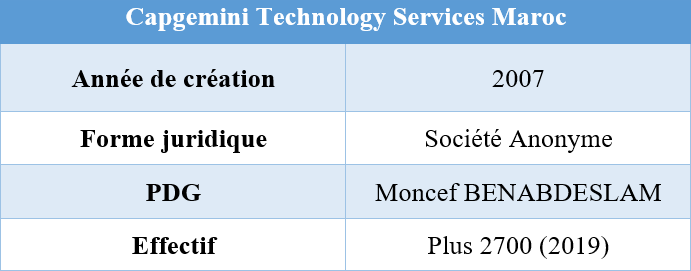
\includegraphics[width=0.8\textwidth]{latex_media/media/image4.png}
    \caption{Fiche d'identité de Capgemini Technology Services Maroc}
    \label{fig:fiche-capgemini-ts}
\end{figure}

\textbf{Capgemini Technology} Services Maroc est une entité spécialisée dans la fourniture de services technologiques et d'ingénierie. Depuis sa création, l'entreprise s'est imposée comme un partenaire incontournable pour de nombreuses organisations, grâce à son expertise et à son engagement envers l'innovation et la qualité des services.

\subsection{Organigramme de Capgemini TS Maroc}

Cette fiche présente l'organigramme de \textbf{Capgemini} TS Maroc, mettant en avant les rôles clés et les responsabilités au sein de notre structure. Elle illustre la hiérarchie et les interactions entre les différents départements, tout en soulignant l'importance de la collaboration pour atteindre nos objectifs.

\begin{figure}[htbp]
    \centering
    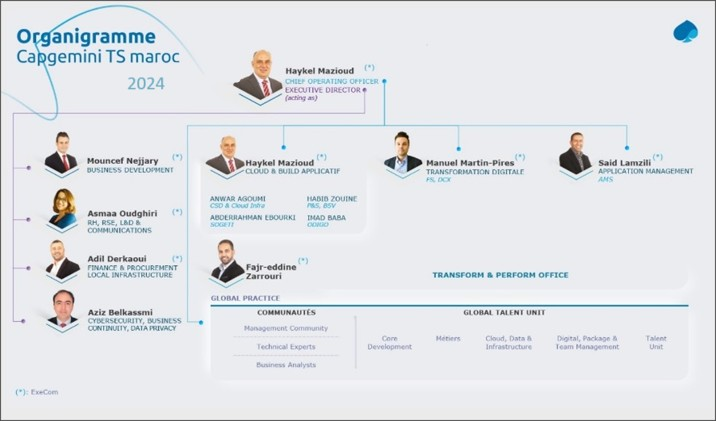
\includegraphics[width=0.9\textwidth]{latex_media/media/image5.jpeg}
    \caption{Organigramme de Capgemini TS Maroc}
    \label{fig:organigramme-capgemini}
\end{figure}

Chaque membre joue un rôle crucial dans le succès de nos projets, et cette représentation visuelle facilite la compréhension de notre organisation.

\subsection{Présentation du DigiCamp}

\begin{figure}[H]
\centering
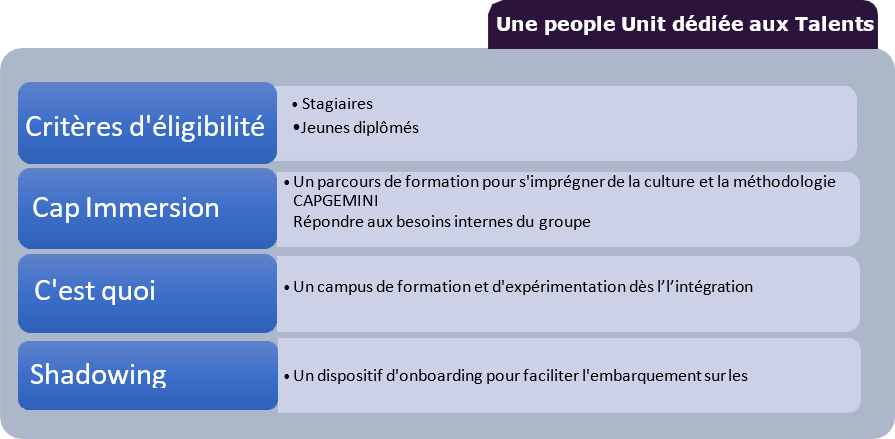
\includegraphics[width=0.8\textwidth]{latex_media/media/image6.png}
\caption{Plateforme Coding Challenge de Capgemini}
\label{fig:coding-challenge-capgemini}
\end{figure}

Dans un contexte où l'évaluation précise des compétences techniques des candidats est cruciale pour le recrutement efficace de talents, la plateforme Coding Challenge de \textbf{Capgemini} représente une réponse stratégique aux défis actuels. Cette plateforme innovante offre aux recruteurs un outil puissant pour évaluer objectivement les capacités des candidats à travers des tests techniques rigoureux. En automatisant une partie du processus de présélection, Coding Challenge permet non seulement de réduire les biais subjectifs associés aux méthodes traditionnelles, mais également d'accélérer significativement le temps nécessaire pour identifier les meilleurs talents. Cet outil s'inscrit dans une stratégie plus large visant à renforcer l'attrait de \textbf{Capgemini} en tant qu'employeur de choix, capable d'attirer et de retenir les profils les plus qualifiés dans le domaine de l'informatique.

DigiCamp a démarré en 2019 avec 39 collaborateurs qui travaillent sur 13 projets en utilisant diverses technologies. Le but est de permettre au talent de prendre son vol vers le staffing dans les projets en passant par les 3 principaux étapes :

\begin{itemize}
\item Cap Immersion.
\item Conditionnement en mode projet.
\item Formation L\&D et accompagnement dans les soft skills, technologies et méthodologie de travail.
\end{itemize}

Un portfolio ambitieux avec des technologies alignées aux besoins et contenant plus de 23 projets dont 15 applications en développement en 2020.

\section{Présentation du projet Quiz Agile}

\subsection{Contexte du projet}

Dans un environnement professionnel où l'agilité est devenue un facteur clé de succès, \textbf{Capgemini} a identifié le besoin de standardiser et d'optimiser l'évaluation des compétences de ses collaborateurs dans ce domaine. Ce besoin s'inscrit dans une stratégie plus large visant à renforcer la culture agile au sein de l'entreprise et à assurer l'excellence opérationnelle des équipes.

L'agilité, avec ses différentes méthodologies (Scrum, Kanban, SAFe, etc.), ses rôles spécifiques (Scrum Master, Product Owner) et ses pratiques (daily stand-up, sprint planning, retrospectives), représente un corpus de connaissances complexe dont la maîtrise est essentielle pour la réussite des projets informatiques modernes.

Jusqu'à présent, l'évaluation des compétences en agilité au sein de \textbf{Capgemini} reposait sur des approches variées et non standardisées : entretiens individuels, observations sur le terrain, ou questionnaires adhoc. Cette diversité d'approches rendait difficile la comparaison des niveaux de compétence entre équipes et limitait la capacité à identifier précisément les besoins de formation.

Par ailleurs, l'entreprise dispose déjà d'une plateforme de formation nommée NEXT, qui propose divers contenus pédagogiques mais ne dispose pas d'un module d'évaluation des compétences intégré. L'articulation entre évaluation et formation représente donc un enjeu majeur pour optimiser les parcours d'apprentissage.

\subsection{Problématique}

Dans le contexte spécifique de l'évaluation des compétences en agilité, le projet \textbf{QUIZ AGILE} vise à répondre à plusieurs problématiques interconnectées :

\begin{itemize}
\item \textbf{Comment standardiser l'évaluation des compétences en agilité à l'échelle de l'entreprise ?} L'absence d'un référentiel commun et d'outils standardisés rend difficile la comparaison des niveaux de compétence entre collaborateurs et entre équipes.
\item \textbf{Comment identifier avec précision les lacunes à combler ?} Les méthodes actuelles ne permettent pas toujours d'analyser finement les domaines spécifiques dans lesquels les collaborateurs ont besoin de renforcer leurs connaissances.
\item \textbf{Comment optimiser les parcours de formation en fonction des résultats d'évaluation ?} Sans lien direct entre évaluation et formation, il est difficile de proposer des parcours d'apprentissage véritablement personnalisés.
\end{itemize}


\begin{figure}[H]
\centering
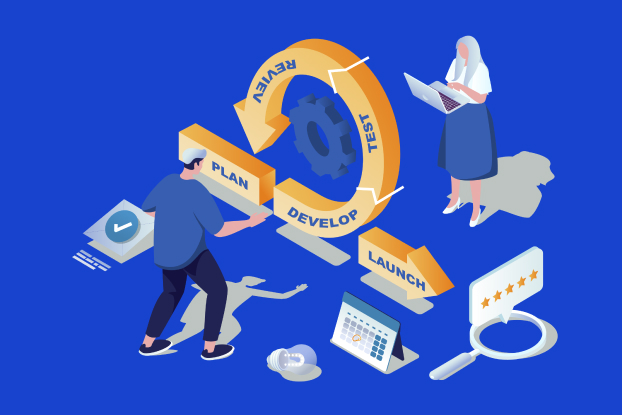
\includegraphics[width=0.8\textwidth]{latex_media/media/image7.jpeg}
\caption{Optimisation des parcours de formation selon les évaluations}
\label{fig:optimisation-parcours}
\end{figure}

\begin{itemize}
\item \textbf{Comment faciliter le suivi de l'évolution des compétences dans le temps ?} L'absence d'historisation des résultats limite la capacité à mesurer les progrès réalisés par les collaborateurs.
\end{itemize}

\subsection{Objectifs du projet}

Le projet \textbf{QUIZ AGILE} poursuit plusieurs objectifs stratégiques :

\begin{itemize}
\item \textbf{Standardiser l'évaluation des compétences en agilité} en proposant un référentiel commun et des outils d'évaluation uniformisés.
\item \textbf{Adapter la formation selon les besoins identifiés} grâce à une analyse précise des résultats et une intégration avec la plateforme de formation NEXT.
\item \textbf{Favoriser l'auto-apprentissage des collaborateurs} en leur permettant d'identifier leurs propres lacunes et de suivre leur progression.
\item \textbf{Fournir aux managers des tableaux de bord détaillés} sur les compétences de leurs équipes pour faciliter la prise de décision.
\item \textbf{Créer une base de connaissances évolutive} pouvant s'étendre à d'autres domaines de compétences au-delà de l'agilité.
\item \textbf{Préparer l'infrastructure pour une future intégration avec des fonctionnalités d'IA} qui permettront d'adapter dynamiquement les quiz en fonction des réponses précédentes.
\end{itemize}

\subsection{Population concernée}

Dans le contexte de la transformation digitale, le projet \textbf{QUIZ AGILE} s'adresse à un écosystème professionnel diversifié au sein de \textbf{Capgemini}, articulé autour de plusieurs catégories de professionnels stratégiques. Les collaborateurs techniques constituent le premier cercle de la population cible, comprenant :

\begin{itemize}
\item Les ingénieurs et développeurs impliqués dans les processus de développement logiciel
\item Les architectes systèmes et les experts en technologies émergentes
\item Les consultants spécialisés en transformation numérique
\end{itemize}

Les professionnels en management représentent un second périmètre crucial, intégrant :
\begin{itemize}
\item Les responsables d'unités opérationnelles
\item Les directeurs de projets technologiques
\item Les leaders en charge du développement organisationnel
\item Les responsables de pratiques métiers
\end{itemize}

L'écosystème de formation et de développement des compétences constitue un troisième groupe stratégique :
\begin{itemize}
\item Les formateurs spécialisés en méthodologies agiles
\item Les responsables du learning \& development
\item Les coaches certifiés en agilité
\item Les experts en gestion des compétences
\end{itemize}

\subsection{Solution proposée}

Face aux défis de l'évolution continue des compétences professionnelles, Quiz Agile émerge comme une solution technologique innovante d'évaluation et de développement des compétences en agilité.

La plateforme se caractérise par une approche méthodologique rigoureuse, articulée autour de plusieurs axes stratégiques :

\subsubsection{Évaluation standardisée des compétences}

Quiz Agile propose un dispositif d'évaluation scientifique et objectif, reposant sur :
\begin{itemize}
\item Des questionnaires à choix multiples hautement paramétrables
\item Un référentiel de compétences normalisé
\item Une approche d'évaluation multicritères
\end{itemize}

\subsubsection{Architecture fonctionnelle innovante}

La solution intègre des fonctionnalités technologiquement avancées :
\begin{itemize}
\item Création de quiz par des experts métiers
\item Passation de tests en environnement numérique sécurisé
\item Analyse approfondie et contextualisation des résultats
\item Recommandations de parcours de formation personnalisés
\item Tableaux de bord décisionnels pour les managers
\end{itemize}

\subsubsection{Intégration technologique et écosystémique}

Quiz Agile se distingue par sa capacité d'intégration :
\begin{itemize}
\item Interconnexion native avec la plateforme de formation NEXT
\item Mécanisme d'authentification unique sécurisé
\item Synchronisation dynamique des données
\item Compatibilité multiplateforme et multiappareils
\end{itemize}

\subsubsection{Bénéfices organisationnels stratégiques}

Quiz Agile vise à générer une valeur ajoutée significative :
\begin{itemize}
\item Identification précise et objective des compétences
\item Personnalisation des trajectoires de développement professionnel
\item Optimisation des investissements en formation
\item Accélération de la transformation culturelle et méthodologique
\end{itemize}

\subsection{Conduite et planification du projet}

La planification est cruciale pour le succès du projet. Elle commence par la conception, où les objectifs et les besoins des utilisateurs sont identifiés. Ensuite, le cadrage fonctionnel et technique établit les fonctionnalités requises et les technologies à utiliser. La phase de codage suit, durant laquelle les développeurs créent le produit selon les spécifications. Ensuite, des tests internes sont effectués pour détecter et corriger les erreurs. Une fois ces tests complétés, le produit est soumis à une validation avec le client pour s'assurer qu'il répond aux attentes. Cette approche structurée garantit un développement efficace et réduit les risques de dérives.

\subsubsection{Intégration et formation continue}

Lors de mon intégration chez \textbf{Capgemini}, j'ai rejoint l'équipe de développement du projet Quiz Agile en tant que Software Engineer Intern. Cette expérience m'a permis de participer activement aux différentes phases de développement de l'application, qui repose sur un écosystème technologique moderne.

Parallèlement, j'ai suivi des formations ciblées sur ces technologies via :
\begin{itemize}
\item La plateforme NEXT de \textbf{Capgemini}
\item La plateforme Udemy
\item Des sessions de formation internes
\end{itemize}

J'ai également complété des formations obligatoires sur :
\begin{itemize}
\item L'éthique professionnelle
\item Le code de conduite de \textbf{Capgemini}
\item La sécurité informatique
\item Les politiques de propriété intellectuelle
\end{itemize}

\subsection{Méthodologie du travail : Agile \& Scrum}

Le projet \textbf{Quiz Agile} a été développé en suivant rigoureusement la méthodologie Agile Scrum, permettant :
\begin{itemize}
\item Un développement itératif et incrémental
\item Une adaptation continue aux besoins
\item Une livraison rapide de valeur métier
\end{itemize}

\cleardoublepage
\section{Conclusion}

Ce premier chapitre a permis de dresser un panorama de \textbf{Capgemini}, de ses activités et de ses engagements, tout en soulignant le rôle central de l'innovation dans ses projets de transformation numérique.

L'analyse du contexte a mis en évidence les limites des processus actuels d'évaluation des compétences en agilité : lenteur, subjectivité, difficulté de standardisation et manque d'outils d'analyse. Ces constats révèlent la nécessité de disposer d'une solution plus rapide, objective et accessible.

Le projet \textbf{QUIZ AGILE} s'inscrit dans cette perspective en proposant une application web intégrée utilisant des technologies modernes. Cette solution vise à améliorer l'évaluation des compétences, faciliter l'adaptation des formations et fournir des outils d'analyse performants, tout en offrant une alternative innovante et efficace aux processus traditionnels.

% ============================================
% CHAPITRE 2 - Analyse et Spécification des besoins
% ============================================

\cleardoublepage
\thispagestyle{empty}
\begin{center}
    \vspace*{4cm}
    {\Huge \textbf{Chapitre 2}}\\[1.5cm]
    {\LARGE \textbf{Analyse et Spécification des besoins}}
\end{center}
\cleardoublepage

\refstepcounter{chapter}
\addcontentsline{toc}{chapter}{Chapitre \thechapter: Analyse et Spécification des besoins}
\markboth{Chapitre \thechapter: Analyse et Spécification des besoins}{}
\setcounter{section}{0}

\section{Introduction}

La phase de conception et de modélisation constitue une étape cruciale
dans le cycle de développement du projet Quiz Agile. Elle permet de
traduire les besoins identifiés lors de l'analyse
préliminaire en une architecture technique et fonctionnelle cohérente.
Ce chapitre présente de manière détaillée l'ensemble des
travaux de conception réalisés, depuis l'analyse des
besoins jusqu'aux choix d'architecture
technique. Nous y aborderons successivement l'analyse
des exigences fonctionnelles et non fonctionnelles,
l'identification des acteurs du système, la modélisation
conceptuelle à travers différents diagrammes UML, et enfin les choix
techniques qui ont guidé l'implémentation du projet.
Cette démarche méthodique vise à garantir que le système final réponde
parfaitement aux attentes des utilisateurs tout en
s'inscrivant dans une architecture évolutive et
maintenable.

\section{Exigences fonctionnelles}

Les exigences fonctionnelles du projet Quiz Agile ont été établies à partir des besoins exprimés par les parties prenantes et des objectifs stratégiques de l'entreprise. Ces exigences définissent les fonctionnalités que le système doit offrir pour répondre aux attentes des utilisateurs.

\subsection{Gestion des utilisateurs}

\begin{itemize}
\item Authentification des utilisateurs avec différents rôles (Administrateur, Coach, Collaborateur)
\item Gestion des profils utilisateurs (création, modification, suppression)
\item Attribution et gestion des droits d'accès selon les rôles
\end{itemize}

\subsection{Gestion des quiz}

\begin{itemize}
\item Création de quiz par les coachs avec titre, description et paramètres
\item Configuration des quiz (durée, nombre de tentatives autorisées, seuil de réussite)
\item Importation et exportation de questions au format standardisé
\item Catégorisation des quiz par thématique et niveau de difficulté
\item Génération d'URL de partage pour diffusion aux collaborateurs
\end{itemize}

\subsection{Gestion des questions}

\begin{itemize}
\item Création de questions de différents types (QCM, vrai/faux, réponses multiples)
\item Association d'options de réponse avec indication des réponses correctes
\item Attribution d'un niveau de difficulté et de mots-clés aux questions
\item Réutilisation des questions dans différents quiz
\item Suggestion intelligente de questions basée sur l'historique et les thématiques
\end{itemize}

\subsection{Passage des quiz}

\begin{itemize}
\item Interface intuitive pour répondre aux questions
\item Chronomètre pour respecter la durée impartie
\item Navigation entre les questions
\item Possibilité de marquer des questions pour y revenir plus tard
\end{itemize}

\subsection{Évaluation et résultats}

\begin{itemize}
\item Calcul automatique des scores
\item Affichage des réponses correctes et des explications après soumission
\item Génération de rapports détaillés pour les participants
\item Attribution de badges et récompenses selon les performances
\item Historique des tentatives et progression dans le temps
\end{itemize}

\subsection{Analyse et reporting}

\begin{itemize}
\item Tableau de bord pour les coachs avec statistiques globales
\item Analyse des performances par équipe, thématique ou question
\item Identification des points forts et des axes d'amélioration
\item Exportation des résultats pour analyse externe
\item Recommandations personnalisées de formation
\end{itemize}

\subsection{Intégration avec la plateforme NEXT}

\begin{itemize}
\item Authentification unique (SSO) entre Quiz Agile et NEXT
\item Synchronisation des données utilisateurs
\item Intégration des quiz dans les parcours de formation NEXT
\item Partage des résultats avec la plateforme NEXT
\end{itemize}

\section{Cartographie fonctionnelle}

\begin{figure}[H]
\centering
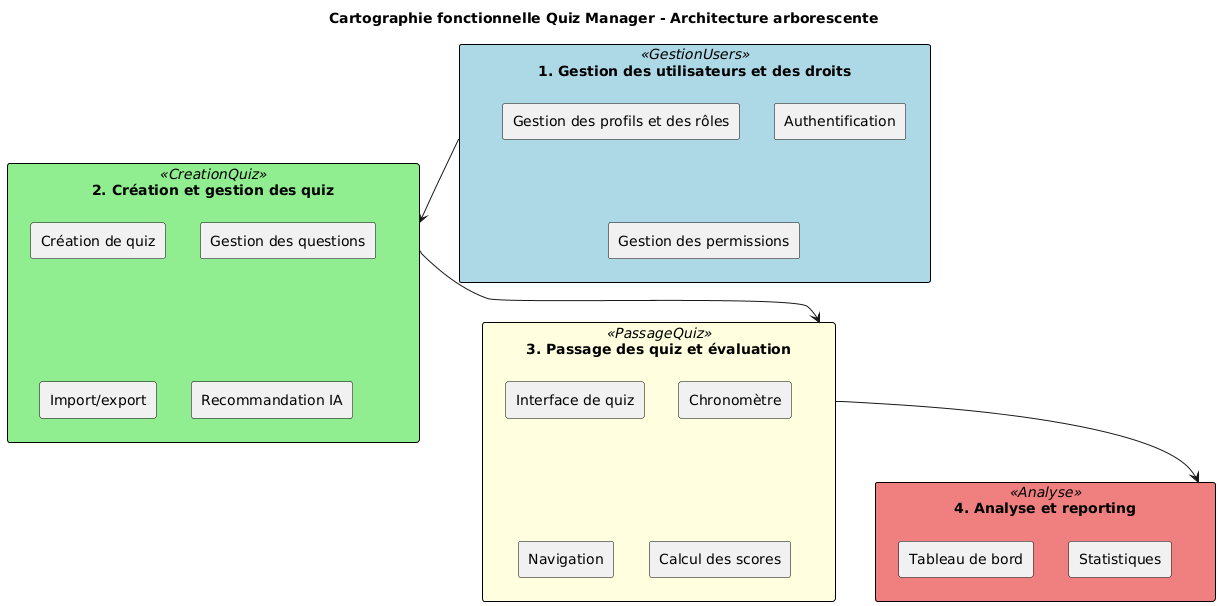
\includegraphics[width=0.8\textwidth]{latex_media/media/image11.png}
\caption{Cartographie fonctionnelle du système Quiz Agile}
\label{fig:cartographie-fonctionnelle}
\end{figure}

La cartographie fonctionnelle ci-dessus présente une vue d'ensemble des principales fonctionnalités du système Quiz Agile et leurs relations.

Cette cartographie met en évidence les quatre grands modules fonctionnels du système :
\begin{itemize}
\item Module de gestion des utilisateurs et des droits
\item Module de création et gestion des quiz
\item Module de passage des quiz et évaluation
\item Module d'analyse et de reporting
\end{itemize}

\section{Spécifications Non Fonctionnelles}

Les exigences non fonctionnelles définissent les critères de qualité et les contraintes techniques que le système doit respecter.

\subsection{Performance}

\begin{itemize}
\item Temps de réponse inférieur à 2 secondes pour les opérations courantes
\item Capacité à gérer simultanément jusqu'à 200 utilisateurs actifs
\item Optimisation des requêtes de base de données pour minimiser la latence
\item Mise en cache des données fréquemment accédées
\end{itemize}

\subsection{Sécurité}

\begin{itemize}
\item Protection des données personnelles conformément au RGPD
\item Authentification sécurisée avec support de l'authentification à deux facteurs
\item Chiffrement des données sensibles en transit et au repos
\item Journalisation des actions critiques pour audit
\item Protection contre les attaques courantes (injection SQL, XSS, CSRF)
\end{itemize}

\subsection{Disponibilité et fiabilité}

\begin{itemize}
\item Disponibilité du système 99,9\% du temps (hors maintenance planifiée)
\item Sauvegarde quotidienne des données avec rétention de 30 jours
\item Plan de reprise d'activité avec un RTO (Recovery Time Objective) de 4 heures
\item Mécanismes de détection et de notification des erreurs
\end{itemize}

\subsection{Maintenabilité}

\begin{itemize}
\item Architecture modulaire facilitant l'évolution du système
\item Documentation complète du code et de l'architecture
\item Tests automatisés couvrant au moins 80\% du code
\item Respect des standards de codage et des bonnes pratiques
\end{itemize}

\subsection{Scalabilité}

\begin{itemize}
\item Architecture permettant une montée en charge horizontale
\item Conception adaptée à une future migration vers les microservices
\item Séparation claire des responsabilités pour faciliter la distribution
\end{itemize}

\subsection{Utilisabilité}

\begin{itemize}
\item Interface utilisateur intuitive et responsive
\item Support multilingue (français et anglais dans un premier temps)
\item Accessibilité conforme aux normes WCAG 2.1 niveau AA
\item Compatibilité avec les principaux navigateurs (Chrome, Firefox, Safari, Edge)
\item Support des appareils mobiles et tablettes
\end{itemize}

\subsection{Interopérabilité}

\begin{itemize}
\item API RESTful documentée pour l'intégration avec des systèmes tiers
\item Support des formats d'échange standards (JSON, XML)
\item Mécanismes d'import/export de données
\end{itemize}

\begin{figure}[H]
\centering
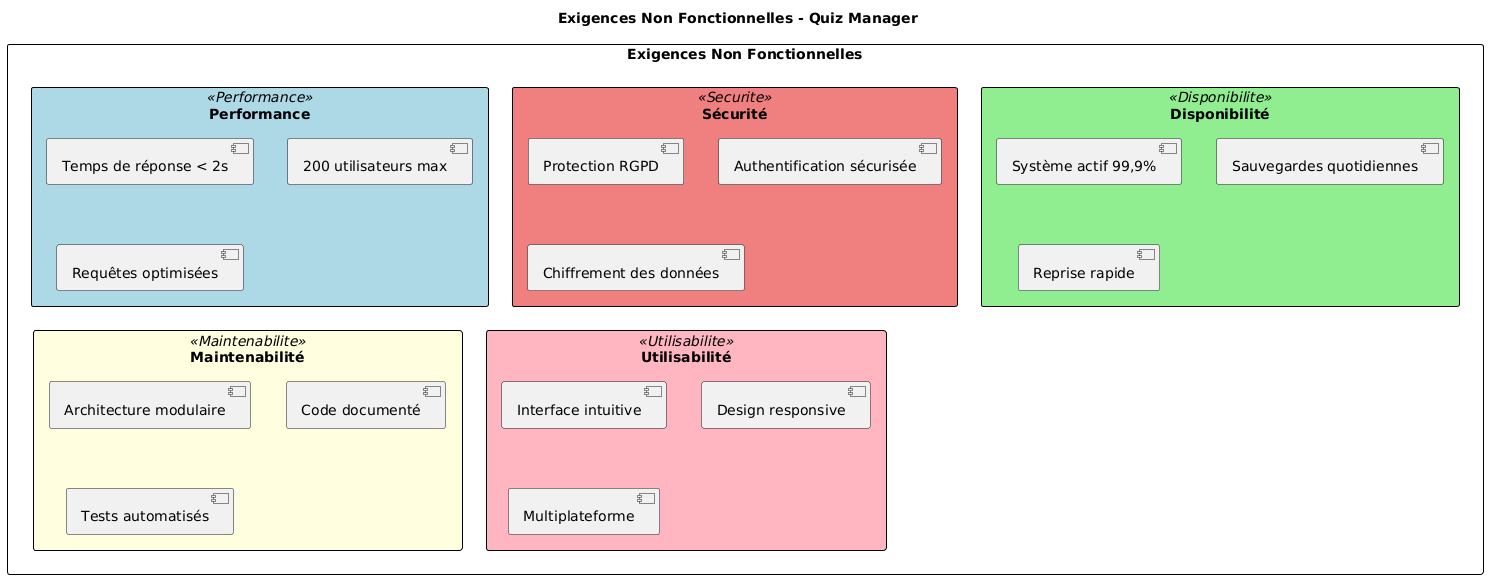
\includegraphics[width=0.9\textwidth]{latex_media/media/image12.png}
\caption{Mécanismes d'import/export de données}
\label{fig:import-export-donnees}
\end{figure}

\section{Analyse des Acteurs et des Cas d'Utilisation}

L'identification des acteurs et de leurs rôles est une étape cruciale dans la conception d'une application. Elle permet de comprendre les besoins spécifiques de chaque utilisateur et de créer une expérience utilisateur optimale. En définissant clairement les rôles et les fonctionnalités associées à chaque type d'utilisateur, on peut garantir que l'application répond aux attentes de chacun et facilite les interactions entre les différents acteurs.

\subsection{Identification des acteurs}

Un acteur est l'idéalisation d'un rôle joué par une personne, un matériel ou un logiciel qui interagit directement avec le système en question. Il peut consulter et / ou modifier directement l'état du système en émettant ou recevant des messages susceptibles d'être porteurs de données.

\begin{figure}[H]
\centering
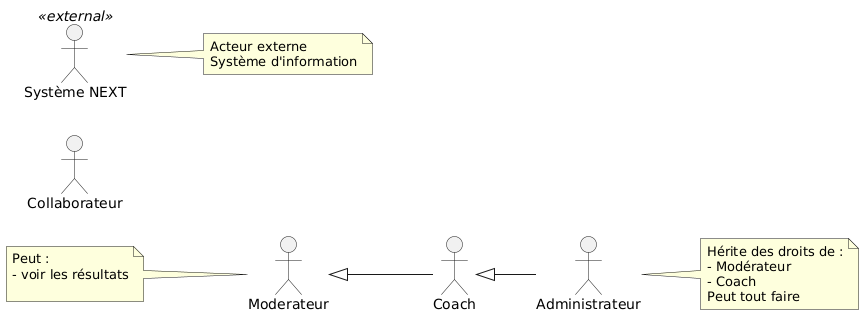
\includegraphics[width=0.9\textwidth]{latex_media/media/image13.png}
\caption{Acteurs principaux du système Quiz Agile}
\label{fig:acteurs-principaux}
\end{figure}

Dans le cadre du projet QUIZ AGILE, plusieurs acteurs clés interagissent avec l'application mobile et la plateforme web. Voici une description de chacun d'eux :

\subsubsection{Administrateur}

\begin{itemize}
\item Responsable de la configuration globale du système
\item Gère les utilisateurs et leurs droits
\item Supervise l'ensemble des activités sur la plateforme
\item Accède aux statistiques globales et aux journaux d'audit
\end{itemize}

\subsubsection{Coach}

\begin{itemize}
\item Crée et gère les quiz et les questions
\item Configure les paramètres des évaluations
\item Analyse les résultats des collaborateurs
\item Identifie les besoins en formation
\item Génère des rapports d'analyse
\end{itemize}

\subsubsection{Collaborateur}

\begin{itemize}
\item Passe les quiz d'évaluation
\item Consulte ses résultats et son historique
\item Suit sa progression dans le temps
\item Reçoit des recommandations personnalisées
\end{itemize}

\subsubsection{Système NEXT}

\begin{itemize}
\item Échange des données avec Quiz Agile
\item Authentifie les utilisateurs via SSO
\item Intègre les quiz dans les parcours de formation
\item Récupère les résultats des évaluations
\end{itemize}

\subsection{Diagramme de Cas d'Utilisation}

Le diagramme de cas d'utilisation est un outil d'analyse puissant qui permet de visualiser les différents cas d'utilisation de l'application et les fonctionnalités associées aux interactions avec les acteurs, offrant ainsi une compréhension globale des besoins des utilisateurs et des objectifs du système.

\begin{figure}[htbp]
    \centering
    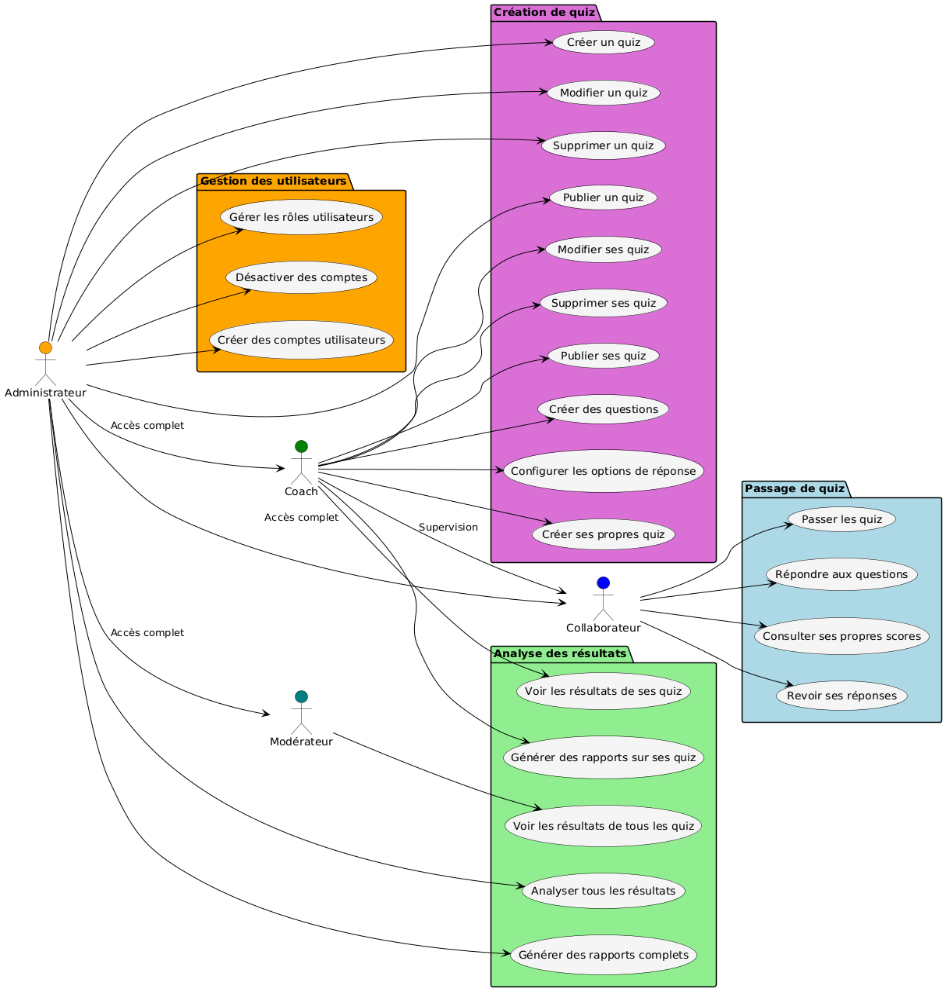
\includegraphics[width=0.7\textwidth]{latex_media/media/image14.png}
    \caption{Diagramme de cas d'utilisation du système Quiz Agile}
    \label{fig:cas-utilisation}
\end{figure}

Le diagramme de cas d'utilisation ci-dessus illustre les principales interactions entre les acteurs et le système Quiz Agile. Le diagramme met en évidence les actions principales accessibles aux différents acteurs après authentification. Cette modélisation permet de comprendre les interactions et les périmètres de responsabilité au sein de l'application Quiz Agile.

\subsection{Tableau Récapitulatif des Cas d'Utilisation}

Ce tableau récapitulatif présente les principaux cas d'utilisation du système \textbf{Quiz Agile}, organisés par domaine fonctionnel. Il détaille les actions clés, les acteurs impliqués (Administrateur, Coach, Collaborateur), et une brève description de chaque fonctionnalité.

\begin{longtable}[]{@{}
  >{\raggedright\arraybackslash}p{(\columnwidth - 6\tabcolsep) * \real{0.2898}}
  >{\raggedright\arraybackslash}p{(\columnwidth - 6\tabcolsep) * \real{0.2367}}
  >{\raggedright\arraybackslash}p{(\columnwidth - 6\tabcolsep) * \real{0.2367}}
  >{\raggedright\arraybackslash}p{(\columnwidth - 6\tabcolsep) * \real{0.2367}}@{}}
\toprule()
\cellcolor{capgeminiblue}\textcolor{white}{\textbf{Domaine}} & \cellcolor{capgeminiblue}\textcolor{white}{\textbf{Cas d'Utilisation}} & \cellcolor{capgeminiblue}\textcolor{white}{\textbf{Acteurs Principaux}} & \cellcolor{capgeminiblue}\textcolor{white}{\textbf{Description}} \\
\midrule()
\endhead
\multirow{3}{*}{Gestion des Utilisateurs} & Créer des comptes & Administrateur & Permettre la création et l'initialisation de nouveaux comptes utilisateurs \\
& Gérer les rôles & Administrateur & Attribuer et modifier les permissions des utilisateurs \\
& Désactiver des comptes & Administrateur & Gérer l'accès et la sécurité du système \\
\multirow{4}{*}{Création de Quiz} & Créer un quiz & Coach & Développer de nouveaux questionnaires \\
& Modifier un quiz & Coach & Mettre à jour le contenu existant \\
& Supprimer un quiz & Coach & Retirer des questionnaires obsolètes \\
& Publier un quiz & Coach & Rendre un quiz accessible aux collaborateurs \\
\multirow{3}{*}{Passage de Quiz} & Passer un quiz & Collaborateur & Réaliser un questionnaire \\
& Répondre aux questions & Collaborateur & Compléter les différentes étapes du quiz \\
& Consulter ses scores & Collaborateur & Visualiser ses performances \\
\multirow{2}{*}{Analyse des Résultats} & Analyser les résultats & Coach/Administrateur & Examiner les performances globales \\
& Générer des rapports & Coach/Administrateur & Produire des analyses détaillées \\
\bottomrule()
\end{longtable}

\begin{center}
\textbf{Tableau 4 :} Tableau récapitulatif des cas d'utilisation
\end{center}

\section{Description détaillée des principaux cas d'utilisation}

\subsection{Cas d'utilisation : Créer un quiz}

Le tableau ci-dessous détaille le processus complet de création d'un quiz, depuis l'initiation par l'administrateur jusqu'à la génération de l'URL partageable, en incluant les scénarios d'erreur et les contraintes techniques :

\begin{longtable}[]{@{}
  >{\raggedright\arraybackslash}p{(\columnwidth - 2\tabcolsep) * \real{0.3329}}
  >{\raggedright\arraybackslash}p{(\columnwidth - 2\tabcolsep) * \real{0.6671}}@{}}
\toprule()
\begin{minipage}[b]{\linewidth}\raggedright
Élément
\end{minipage} & \begin{minipage}[b]{\linewidth}\raggedright
Description Détaillée
\end{minipage} \\
\midrule()
\endhead
Titre & \textbf{Création d'un Quiz en Ligne} \\
Acteur Principal & \textbf{Administrateur/Créateur de Quiz} \\
Objectif & \textbf{Créer un quiz interactif} \\
Préconditions & \textbf{- Compte administrateur valide} \\
& \textbf{- Accès à l'outil de création de quiz} \\
Flux Principal & \textbf{1. Initiation de la création de quiz} \\
& \textbf{2. Remplissage des détails de base (titre, description)} \\
& \textbf{3. Sélection de la méthode de question} \\
& \textbf{4. Définition des paramètres du quiz} \\
& \textbf{5. Validation du quiz} \\
& \textbf{6. Création d'une URL partageable} \\
Actions du Système & \textbf{- Authentification} \\
& \textbf{- Enregistrement des détails du quiz} \\
& \textbf{- Génération des questions selon la méthode choisie} \\
& \textbf{- Validation des questions et des options} \\
& \textbf{- Création de l'URL de partage} \\
Scénarios Alternatifs & \textbf{- Échec de validation du quiz} \\
& \textbf{- Modification des questions après validation} \\
Gestion des Erreurs & \textbf{- Messages d'erreur en cas de problèmes} \\
& \textbf{- Sauvegarde des données en cas de déconnexion} \\
Postconditions & \textbf{- Quiz créé et prêt à être partagé} \\
Règles et Contraintes & \textbf{- Vérification des droits d'accès} \\
& \textbf{- Respect des délais de création} \\
Résultat Final & \textbf{- Quiz enregistré dans la base de données} \\
& \textbf{- Notification de création réussie} \\
Interactions Additionnelles & \textbf{- Possibilité de prévisualiser le quiz} \\
& \textbf{- Consultation des statistiques de création} \\
Critères de Succès & \textbf{- Quiz créé avec succès} \\
& \textbf{- Validation des paramètres du quiz} \\
\bottomrule()
\end{longtable}

\begin{center}
\textbf{Tableau 5 :} Cas d'utilisation : Créer un quiz
\end{center}

\subsection{Cas d'utilisation : Passer un quiz}

Le tableau ci-dessous présente le déroulement optimisé pour le passage d'un quiz par un collaborateur, mettant l'accent sur l'expérience utilisateur, les mécanismes de sauvegarde et l'analyse des performances post-quiz :

\begin{longtable}[]{@{}
  >{\raggedright\arraybackslash}p{(\columnwidth - 2\tabcolsep) * \real{0.3684}}
  >{\raggedright\arraybackslash}p{(\columnwidth - 2\tabcolsep) * \real{0.6316}}@{}}
\toprule()
\begin{minipage}[b]{\linewidth}\raggedright
Élément
\end{minipage} & \begin{minipage}[b]{\linewidth}\raggedright
Description Détaillée
\end{minipage} \\
\midrule()
\endhead
Titre & Réalisation d'un Quiz en Ligne \\
Acteur Principal & Collaborateur \\
Objectif & Compléter un quiz interactivement \\
Préconditions & \begin{minipage}[t]{\linewidth}\raggedright
- Compte utilisateur valide\\
- Quiz accessible\\
- Connexion internet stable\strut
\end{minipage} \\
Flux Principal & \begin{minipage}[t]{\linewidth}\raggedright
1. Accès via URL partagée\\
2. Lecture des instructions\\
3. Démarrage du quiz\\
4. Navigation entre questions\\
5. Réponse aux questions\\
6. Soumission des réponses\strut
\end{minipage} \\
Actions du Système & \begin{minipage}[t]{\linewidth}\raggedright
- Authentification\\
- Initialisation du chronomètre\\
- Enregistrement des réponses\\
- Calcul du score\\
- Génération du feedback\strut
\end{minipage} \\
Scénarios Alternatifs & \begin{minipage}[t]{\linewidth}\raggedright
- Expiration du temps\\
- Soumission automatique\\
- Feedback immédiat possible\\
- Réponses partielles acceptées\strut
\end{minipage} \\
Gestion des Erreurs & \begin{minipage}[t]{\linewidth}\raggedright
- Sauvegarde partielle en cas de déconnexion\\
- Blocage en cas d'accès non autorisé\\
- Messages explicatifs d'erreur\strut
\end{minipage} \\
Postconditions & \begin{minipage}[t]{\linewidth}\raggedright
- Réponses enregistrées\\
- Score calculé\\
- Résultats disponibles\\
- Analyse détaillée générée\strut
\end{minipage} \\
Règles et Contraintes & \begin{minipage}[t]{\linewidth}\raggedright
- Temps limité\\
- Une seule tentative\\
- Pas de retour arrière après soumission\\
- Vérification des droits d'accès\strut
\end{minipage} \\
Résultat Final & \begin{minipage}[t]{\linewidth}\raggedright
- Affichage du score\\
- Présentation du feedback\\
- Analyse des performances\strut
\end{minipage} \\
Interactions Additionnelles &
\begin{minipage}[t]{\linewidth}\raggedright
- Possibilité de voir les détails du quiz\\
- Consultation du rapport détaillé\\
- Comparaison éventuelle avec d'autres participants\strut
\end{minipage} \\
Critères de Succès & \begin{minipage}[t]{\linewidth}\raggedright
- Complétion du quiz\\
- Compréhension des résultats\\
- Expérience utilisateur fluide\strut
\end{minipage} \\
\bottomrule()
\end{longtable}

\begin{center}
\textbf{Tableau 6 :} Cas d'utilisation : Passer un quiz
\end{center}

\section{Architecture monolithique}

Dans les projets informatiques, une des premières grandes étapes techniques est de faire des choix architecturaux : « Comment organiser l'application ? » Deux solutions architecturales principales se présentent : l'architecture monolithique et l'architecture micro-services.

L'architecture monolithique consiste à développer l'application comme une unité unique, où tous les composants sont interconnectés et déployés ensemble. Cette approche peut simplifier le développement initial et la gestion des déploiements, mais elle peut devenir difficile à maintenir et à faire évoluer à mesure que l'application croît.

En revanche, l'architecture micro-services divise l'application en services indépendants, chacun responsable d'une fonctionnalité spécifique. Cela permet une plus grande flexibilité, une scalabilité améliorée et une meilleure gestion des équipes, car chaque service peut être développé, déployé et mis à jour indépendamment.

Cependant, cette approche nécessite une gestion plus complexe des communications entre services et une attention particulière à la sécurité et à la résilience globale du système.

\begin{figure}[H]
\centering
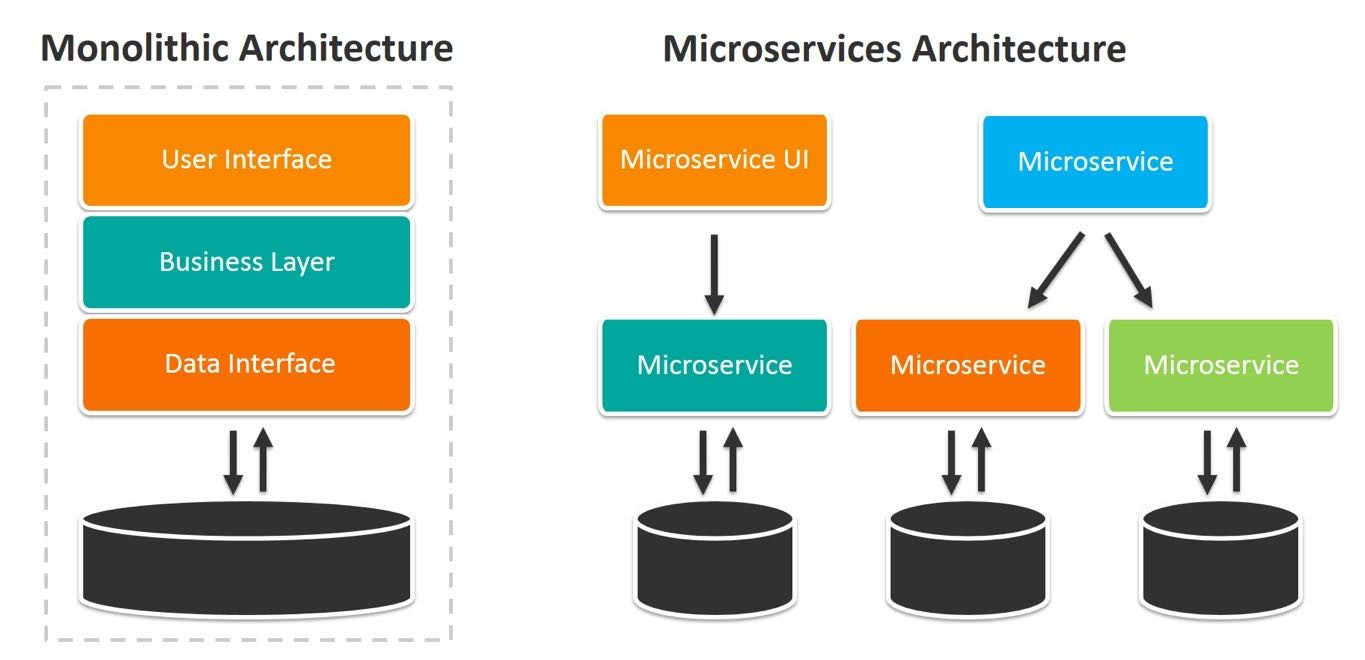
\includegraphics[width=0.8\textwidth]{latex_media/media/image15.jpeg}
\caption{Comparaison entre architecture monolithique et microservices}
\label{fig:comparaison-architectures}
\end{figure}

Le choix entre ces deux architectures dépendra des besoins spécifiques du projet, de l'équipe en place et des objectifs à long terme.

Pour le cas de la solution QUIZ AGILE, nous avons opté pour l'architecture monolithique. Ce choix nous permet, durant les premières phases du projet, de simplifier la charge cognitive liée à la gestion du code et au déploiement. En structurant l'application comme une unité unique, nous pouvons livrer tout le contenu du monolithe à la fois, ce qui facilite le processus de développement et réduit les complexités associées à l'intégration continue.

Cette approche initiale nous offre également une vue d'ensemble cohérente du projet, permettant aux équipes de se concentrer sur l'implémentation des fonctionnalités sans se soucier des défis d'architecture distribuée. À mesure que le projet évolue et que les besoins se précisent, nous pourrons envisager une transition vers une architecture micro-services, si nécessaire, pour répondre à des exigences de scalabilité ou de maintenance plus stricte.

\subsection{Conclusion}

Le choix d'une architecture monolithique pour cette première phase du projet se justifie par sa simplicité de déploiement et de maintenance, tout en restant compatible avec une éventuelle migration vers une architecture micro-services si les besoins évoluent (scalabilité, modularité accrue).

\subsection{Évaluation et résultats}

\begin{itemize}
\item Calcul automatique des scores
\item Affichage des réponses correctes et des explications après soumission
\item Génération de rapports détaillés pour les participants
\item Attribution de badges et récompenses selon les performances
\item Historique des tentatives et progression dans le temps
\end{itemize}

\subsection{Analyse et reporting}

\begin{itemize}
\item Tableau de bord pour les coachs avec statistiques globales
\item Analyse des performances par équipe, thématique ou question
\item Identification des points forts et des axes d'amélioration
\item Exportation des résultats pour analyse externe
\item Recommandations personnalisées de formation
\end{itemize}

\subsection{Intégration avec la plateforme NEXT}

\begin{itemize}
\item Authentification unique (SSO) entre Quiz Agile et NEXT
\item Synchronisation des données utilisateurs
\item Intégration des quiz dans les parcours de formation NEXT
\item Partage des résultats avec la plateforme NEXT
\end{itemize}

\section{Spécifications non fonctionnelles}

Les exigences non fonctionnelles définissent les critères de qualité et
les contraintes techniques que le système doit respecter.

\subsection{Performance}

\begin{itemize}
\item Temps de réponse inférieur à 2 secondes pour les opérations courantes
\item Capacité à gérer simultanément jusqu'à 200 utilisateurs actifs
\item Optimisation des requêtes de base de données pour minimiser la latence
\item Mise en cache des données fréquemment accédées
\end{itemize}

\subsection{Sécurité}

\begin{itemize}
\item Protection des données personnelles conformément au RGPD
\item Authentification sécurisée avec support de l'authentification à deux facteurs
\item Chiffrement des données sensibles en transit et au repos
\item Journalisation des actions critiques pour audit
\item Protection contre les attaques courantes (injection SQL, XSS, CSRF)
\end{itemize}

\subsection{Disponibilité et fiabilité}

\begin{itemize}
\item Disponibilité du système 99,9\% du temps (hors maintenance planifiée)
\item Sauvegarde quotidienne des données avec rétention de 30 jours
\item Plan de reprise d'activité avec un RTO (Recovery Time Objective) de 4 heures
\item Mécanismes de détection et de notification des erreurs
\end{itemize}

\subsection{Maintenabilité}

\begin{itemize}
\item Architecture modulaire facilitant l'évolution du système
\item Documentation complète du code et de l'architecture
\item Tests automatisés couvrant au moins 80\% du code
\item Respect des standards de codage et des bonnes pratiques
\end{itemize}

\subsection{Utilisabilité}

\begin{itemize}
\item Interface utilisateur intuitive et responsive
\item Support multilingue (français et anglais dans un premier temps)
\item Accessibilité conforme aux normes WCAG 2.1 niveau AA
\item Compatibilité avec les principaux navigateurs (Chrome, Firefox, Safari, Edge)
\item Support des appareils mobiles et tablettes
\end{itemize}

\section{Identification des acteurs}

Dans le cadre du projet QUIZ AGILE, plusieurs acteurs clés interagissent avec l'application. Voici une description de chacun d'eux :

\subsection{Administrateur}

\begin{itemize}
\item Responsable de la configuration globale du système
\item Gère les utilisateurs et leurs droits
\item Supervise l'ensemble des activités sur la plateforme
\item Accède aux statistiques globales et aux journaux d'audit
\end{itemize}

\subsection{Coach}

\begin{itemize}
\item Crée et gère les quiz et les questions
\item Configure les paramètres des évaluations
\item Analyse les résultats des collaborateurs
\item Identifie les besoins en formation
\item Génère des rapports d'analyse
\end{itemize}

\subsection{Collaborateur}

\begin{itemize}
\item Passe les quiz d'évaluation
\item Consulte ses résultats et son historique
\item Suit sa progression dans le temps
\item Reçoit des recommandations personnalisées
\end{itemize}

\subsection{Système NEXT}

\begin{itemize}
\item Échange des données avec Quiz Agile
\item Authentifie les utilisateurs via SSO
\item Intègre les quiz dans les parcours de formation
\item Récupère les résultats des évaluations
\end{itemize}

\section{Diagramme de cas d'utilisation}

\begin{figure}[htbp]
    \centering
    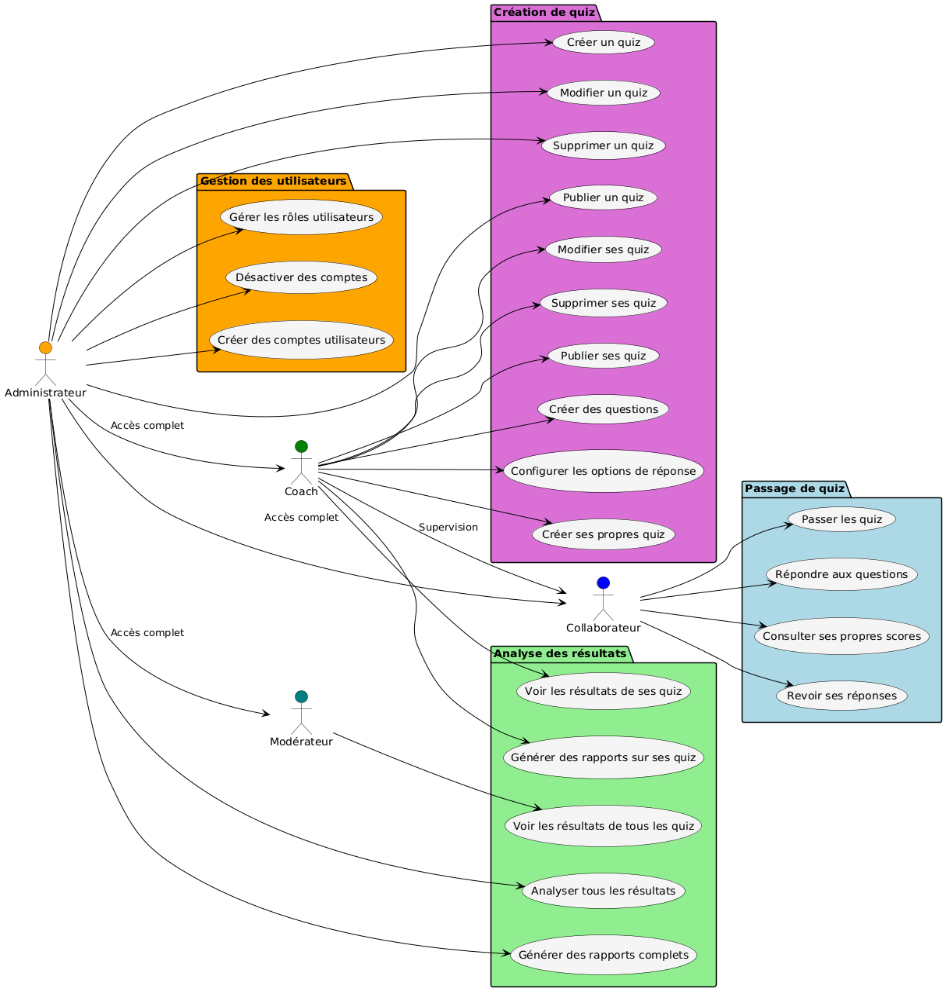
\includegraphics[width=0.9\textwidth]{latex_media/media/image14.png}
    \caption{Diagramme de cas d'utilisation du système Quiz Agile}
    \label{fig:cas-utilisation}
\end{figure}

Le diagramme de cas d'utilisation ci-dessus illustre les principales interactions entre les acteurs et le système Quiz Agile. Cette modélisation permet de comprendre les interactions et les périmètres de responsabilité au sein de l'application Quiz Agile.

\section{Conclusion}

Ce chapitre a présenté l'analyse détaillée des besoins fonctionnels et non-fonctionnels du projet Quiz Agile. L'identification claire des acteurs et de leurs rôles, ainsi que la modélisation des cas d'utilisation, fournissent une base solide pour la conception et le développement du système. Cette approche méthodique garantit que la solution finale répondra aux attentes de tous les utilisateurs tout en respectant les contraintes techniques et de qualité requises.

% ============================================
% CHAPITRE 3 - Conception et Mise en place du système
% ============================================

\cleardoublepage
\thispagestyle{empty}
\begin{center}
    \vspace*{4cm}
    {\Huge \textbf{Chapitre 3}}\\[1.5cm]
    {\LARGE \textbf{Conception et Mise en place du système}}
\end{center}
\cleardoublepage

\refstepcounter{chapter}
\addcontentsline{toc}{chapter}{Chapitre \thechapter: Conception et Mise en place du système}
\markboth{Chapitre \thechapter: Conception et Mise en place du système}{}
\setcounter{section}{0}

\section{Introduction}

La conception constitue une étape clé entre la spécification des besoins et l'implémentation. Elle permet de représenter, sous forme de modèles, la structure et le comportement du système afin de garantir sa cohérence, sa robustesse et sa maintenabilité.

Dans le cadre du projet \textbf{QUIZ AGILE}, la conception se décline en deux volets complémentaires :
\begin{itemize}
    \item la \textbf{modélisation dynamique} décrivant les comportements, scénarios et flux de données (diagrammes de séquence et d'activités)
    \item la \textbf{modélisation statique} mettant en avant la structure du système (diagramme de classes et modèle relationnel) ainsi que l'architecture logicielle de déploiement
\end{itemize}

\section{Architecture du système}

\subsection{Architecture logicielle}

L'architecture logicielle du système Quiz Agile repose sur une approche en couches (layered architecture) qui garantit une séparation claire des responsabilités et facilite la maintenance et l'évolutivité du système.

\subsubsection{Architecture 3-tiers}

Le système adopte une architecture 3-tiers classique :

\begin{itemize}
    \item \textbf{Couche Présentation} : Interface utilisateur développée en React
    \item \textbf{Couche Métier} : Logique applicative implémentée avec Spring Boot
    \item \textbf{Couche Données} : Base de données relationnelle MySQL
\end{itemize}

\subsubsection{Patron d'architecture MVC}

L'application respecte le patron Modèle-Vue-Contrôleur (MVC) :

\begin{itemize}
    \item \textbf{Modèle} : Entités JPA et services métier
    \item \textbf{Vue} : Composants React pour l'interface utilisateur
    \item \textbf{Contrôleur} : REST Controllers Spring Boot
\end{itemize}

\subsection{Architecture de déploiement}

L'architecture de déploiement prévoit une séparation entre l'environnement de développement et l'environnement de production, avec des mécanismes de CI/CD pour automatiser les déploiements.

\section{Modélisation UML}

\subsection{Diagramme de classes}

Le diagramme de classes présente les principales entités du système et leurs relations. Les entités principales sont :

\begin{itemize}
    \item \textbf{User} : Représente les utilisateurs du système
    \item \textbf{Quiz} : Modélise les questionnaires
    \item \textbf{Question} : Représente les questions individuelles
    \item \textbf{Answer} : Modélise les réponses possibles
    \item \textbf{Result} : Stocke les résultats des quiz
\end{itemize}

\subsection{Diagramme de séquence}

Les diagrammes de séquence illustrent les interactions entre les différents composants du système pour les cas d'utilisation principaux :

\begin{itemize}
    \item Création d'un quiz
    \item Passage d'un quiz
    \item Consultation des résultats
\end{itemize}

\section{Modèle de données}

\subsection{Modèle conceptuel}

Le modèle conceptuel de données définit les entités principales et leurs relations :

\begin{itemize}
    \item Un utilisateur peut créer plusieurs quiz
    \item Un quiz contient plusieurs questions
    \item Une question peut avoir plusieurs réponses
    \item Un utilisateur peut passer plusieurs quiz
    \item Chaque passage génère un résultat
\end{itemize}

\subsection{Modèle relationnel}

Le modèle relationnel dérive du modèle conceptuel et respecte les formes normales pour éviter la redondance et garantir l'intégrité des données.

\section{Technologies et outils utilisés}

\subsection{Backend - Spring Boot}

Spring Boot a été choisi pour le développement du backend pour ses avantages :

\begin{itemize}
    \item Framework mature et robuste
    \item Configuration automatique
    \item Écosystème riche (Spring Security, Spring Data, etc.)
    \item Support natif des API REST
    \item Facilité de test et de déploiement
\end{itemize}

\subsection{Frontend - React}

React a été sélectionné pour l'interface utilisateur :

\begin{itemize}
    \item Composants réutilisables
    \item Virtual DOM pour les performances
    \item Écosystème riche de bibliothèques
    \item Communauté active et documentation complète
\end{itemize}

\subsection{Base de données - MySQL}

MySQL a été choisi comme SGBD relationnel :

\begin{itemize}
    \item Fiabilité et performance éprouvées
    \item Support transactionnel complet
    \item Outils d'administration matures
    \item Compatibilité avec Spring Data JPA
\end{itemize}

\section{Conclusion}

Ce chapitre a présenté la conception détaillée du système Quiz Agile, depuis l'architecture générale jusqu'aux choix technologiques. Cette approche structurée garantit un système cohérent, maintenable et évolutif, répondant aux exigences fonctionnelles et non-fonctionnelles identifiées.

% ============================================
% CHAPITRE 4 - Réalisation, Tests et Étude Technique
% ============================================

\cleardoublepage
\thispagestyle{empty}
\begin{center}
    \vspace*{4cm}
    {\Huge \textbf{Chapitre 4}}\\[1.5cm]
    {\LARGE \textbf{Réalisation, Tests et Étude Technique}}
\end{center}
\cleardoublepage

\refstepcounter{chapter}
\addcontentsline{toc}{chapter}{Chapitre \thechapter: Réalisation, Tests et Étude Technique}
\markboth{Chapitre \thechapter: Réalisation, Tests et Étude Technique}{}
\setcounter{section}{0}

\section{Introduction}

Ce chapitre détaille la mise en œuvre concrète du projet \textbf{QUIZ AGILE}, depuis la configuration de l'environnement de développement jusqu'aux tests de validation, en passant par l'implémentation des différents modules du système. Chaque étape est illustrée par des exemples de code et des captures d'écran des interfaces développées.

\section{Environnement de développement}

\subsection{Configuration de l'environnement}

L'environnement de développement a été configuré avec les outils suivants :

\begin{itemize}
    \item \textbf{IDE} : IntelliJ IDEA pour le backend, Visual Studio Code pour le frontend
    \item \textbf{Java} : Version 11 LTS
    \item \textbf{Node.js} : Version 16 LTS
    \item \textbf{Base de données} : MySQL 8.0
    \item \textbf{Outils de build} : Maven pour Java, npm pour React
\end{itemize}

\subsection{Structure du projet}

Le projet est organisé en deux modules principaux :

\begin{itemize}
    \item \textbf{quiz-agile-backend} : Application Spring Boot
    \item \textbf{quiz-agile-frontend} : Application React
\end{itemize}

\section{Implémentation du backend}

\subsection{Configuration Spring Boot}

Le backend utilise Spring Boot avec les dépendances suivantes :

\begin{itemize}
    \item Spring Web (pour les API REST)
    \item Spring Data JPA (pour l'accès aux données)
    \item Spring Security (pour l'authentification)
    \item MySQL Connector (pour la base de données)
    \item Validation API (pour la validation des données)
\end{itemize}

\subsection{Modèle de données}

Les entités principales du système ont été implémentées avec JPA :

\begin{itemize}
    \item Entité User pour la gestion des utilisateurs
    \item Entité Quiz pour les questionnaires
    \item Entité Question pour les questions
    \item Entité Answer pour les réponses
    \item Entité Result pour les résultats
\end{itemize}

\subsection{Services métier}

Les services métier implémentent la logique applicative :

\begin{itemize}
    \item UserService pour la gestion des utilisateurs
    \item QuizService pour la gestion des quiz
    \item QuestionService pour la gestion des questions
    \item ResultService pour l'analyse des résultats
\end{itemize}

\subsection{API REST}

L'API REST expose les fonctionnalités via des contrôleurs :

\begin{itemize}
    \item AuthController pour l'authentification
    \item QuizController pour la gestion des quiz
    \item UserController pour la gestion des utilisateurs
    \item ResultController pour l'accès aux résultats
\end{itemize}

\section{Implémentation du frontend}

\subsection{Architecture React}

L'application frontend est structurée avec :

\begin{itemize}
    \item Composants fonctionnels avec React Hooks
    \item React Router pour la navigation
    \item Axios pour les appels API
    \item Material-UI pour l'interface utilisateur
\end{itemize}

\subsection{Gestion d'état}

La gestion d'état utilise :

\begin{itemize}
    \item Context API pour l'état global
    \item useState et useEffect pour l'état local
    \item Custom hooks pour la logique réutilisable
\end{itemize}

\subsection{Composants principaux}

Les composants principaux incluent :

\begin{itemize}
    \item Dashboard pour le tableau de bord
    \item QuizForm pour la création/édition de quiz
    \item QuizPlayer pour le passage des quiz
    \item ResultsView pour l'affichage des résultats
\end{itemize}

\section{Tests et validation}

\subsection{Tests unitaires}

Des tests unitaires ont été implémentés pour :

\begin{itemize}
    \item Les services métier du backend
    \item Les composants React
    \item Les utilitaires et fonctions helper
\end{itemize}

\subsection{Tests d'intégration}

Les tests d'intégration couvrent :

\begin{itemize}
    \item Les API REST
    \item L'accès aux données
    \item Les flux end-to-end principaux
\end{itemize}

\subsection{Tests de performance}

Des tests de charge ont été réalisés pour valider :

\begin{itemize}
    \item La capacité de traitement concurrent
    \item Les temps de réponse sous charge
    \item La stabilité du système
\end{itemize}

\section{Déploiement}

\subsection{Conteneurisation}

L'application a été conteneurisée avec Docker :

\begin{itemize}
    \item Image Docker pour le backend Spring Boot
    \item Image Docker pour le frontend React buildé
    \item Docker Compose pour l'orchestration locale
\end{itemize}

\subsection{Pipeline CI/CD}

Un pipeline CI/CD a été mis en place avec :

\begin{itemize}
    \item Build automatique sur commit
    \item Exécution des tests automatisés
    \item Déploiement automatique en environnement de test
\end{itemize}

\section{Conclusion}

Ce chapitre a détaillé l'implémentation complète du système Quiz Agile. L'approche méthodique adoptée, combinée aux bonnes pratiques de développement et aux tests rigoureux, a permis de livrer une solution robuste et fonctionnelle répondant aux exigences définies.

% ============================================
% CHAPITRE 3 - Conception et Mise en place du projet
% ============================================

\cleardoublepage
\thispagestyle{empty}
\begin{center}
    \vspace*{4cm}
    {\Huge \textbf{Chapitre 3}}\\[1.5cm]
    {\LARGE \textbf{Conception et Mise en place du projet}}
\end{center}
\cleardoublepage

\refstepcounter{chapter}
\addcontentsline{toc}{chapter}{Chapitre \thechapter: Conception et Mise en place du projet}
\markboth{Chapitre \thechapter: Conception et Mise en place du projet}{}
\setcounter{section}{0}

\section{Introduction}

Avant de plonger dans le développement de l'application QUIZ AGILE, une planification rigoureuse et une conception méticuleuse sont essentielles. Cette phase préparatoire, loin d'être une simple formalité, constitue le fondement sur lequel repose le succès du projet. Elle permet de minimiser les risques, d'optimiser les ressources et de garantir que le produit final répondra aux attentes spécifiques des utilisateurs, notamment des collaborateurs et de leurs accompagnateurs.

La modélisation joue un rôle crucial dans ce processus, transformant des concepts abstraits en représentations concrètes. Elle permet de visualiser les fonctionnalités à réaliser, de clarifier les interactions entre les différents éléments et d'offrir une compréhension globale du système. Ce processus est le pont qui relie l'idée initiale à l'application finale, permettant de concrétiser les aspirations en un outil tangible et fonctionnel.

Ce chapitre explore la méthodologie et la réalisation du projet QUIZ AGILE, en mettant l'accent sur les éléments clés de la conception, tels que les diagrammes de cas d'utilisation, les diagrammes de classes et de séquences, ainsi que la structure de la base de données. De plus, nous aborderons les algorithmes qui constituent une fonctionnalité majeure de notre application, facilitant l'interaction et l'engagement des utilisateurs.

\section{Diagramme de classes}

Le diagramme de classes, véritable pierre angulaire de la modélisation objet, se positionne comme un outil incontournable pour la conception et la planification d'architectures logicielles robustes. Il offre une représentation visuelle des classes, de leurs attributs, de leurs méthodes et des relations qui les lient, permettant ainsi une compréhension approfondie de la structure interne du code et de ses interactions complexes.

Le diagramme présenté a joué un rôle crucial dans la communication entre les membres de l'équipe, favorisant une vision commune de l'architecture logicielle et réduisant les risques d'erreurs lors de l'implémentation :

\begin{figure}[H]
\centering
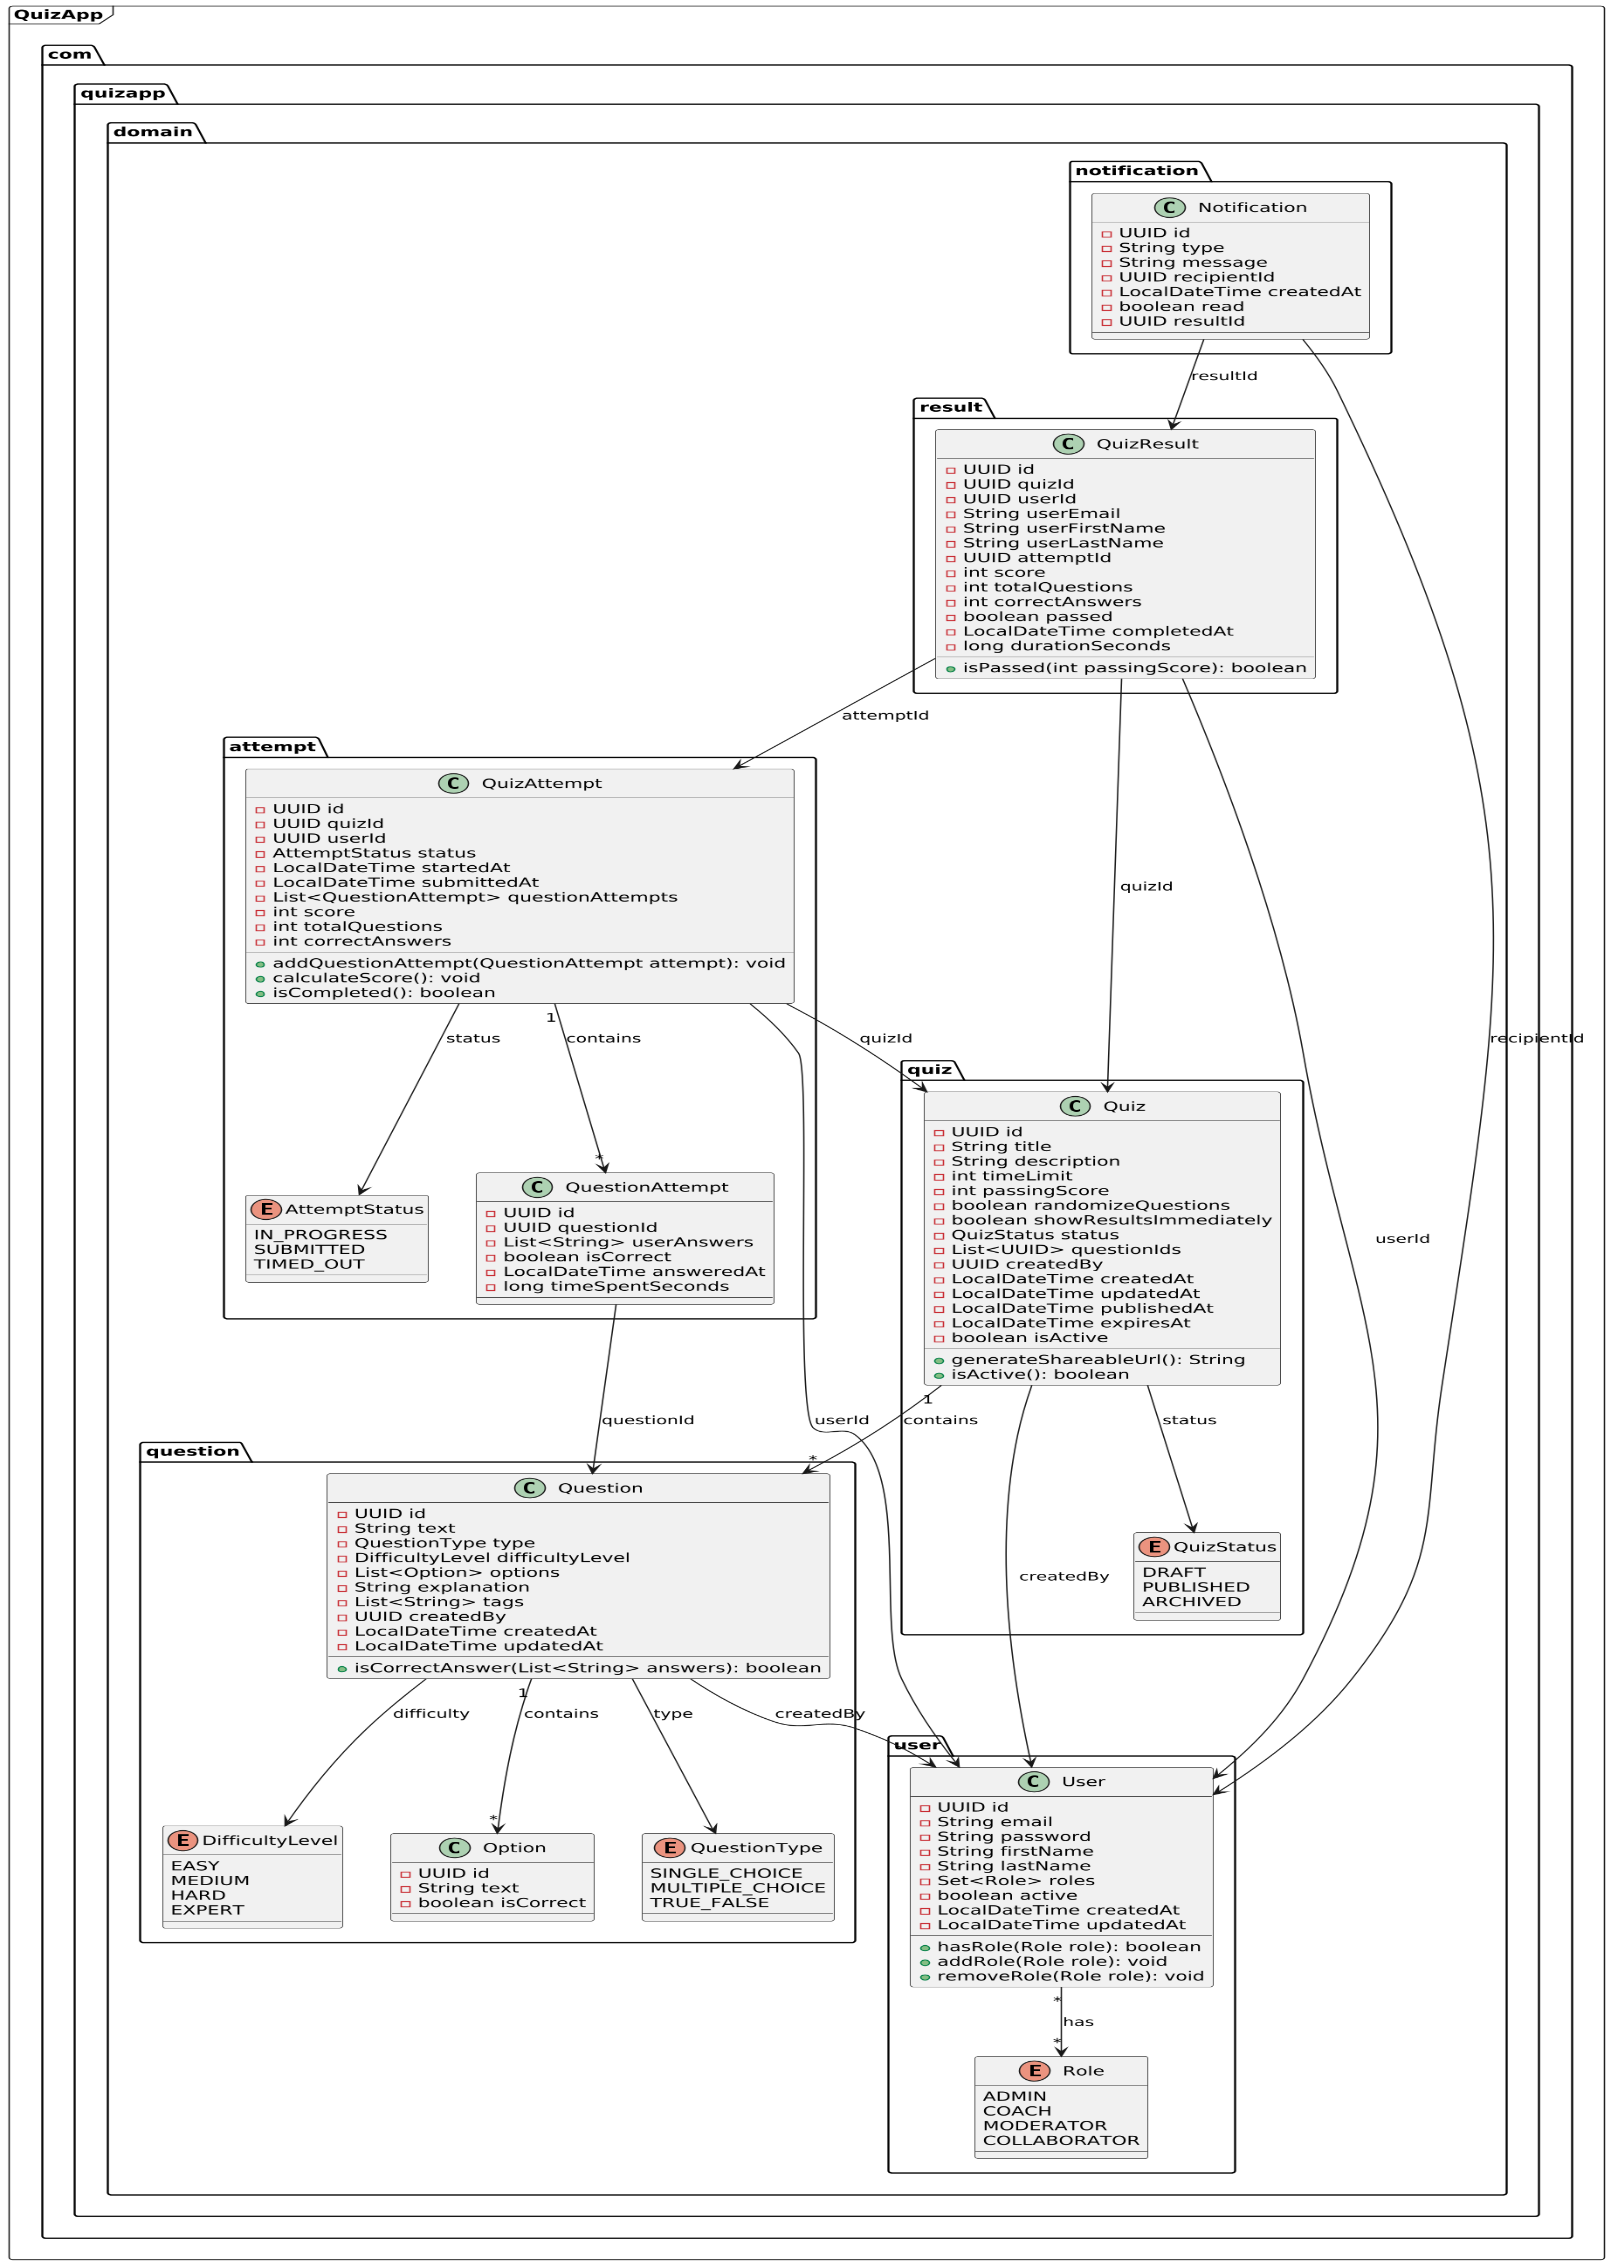
\includegraphics[width=0.9\textwidth]{latex_media/media/image16.png}
\caption{Diagramme de classes du système Quiz Agile}
\label{fig:diagramme-classes}
\end{figure}

Le diagramme représente un système de quiz en ligne avec 6 packages principaux organisés en cadre "\textbf{Agile Quiz}" :

\begin{enumerate}
\item \textbf{User} - Gestion des utilisateurs et rôles
\item \textbf{Question} - Gestion des questions et options
\item \textbf{Quiz} - Gestion des questionnaires
\item \textbf{Attempt} - Suivi des tentatives de quiz
\item \textbf{Result} - Résultats des quiz
\item \textbf{Notification} - Notifications système
\end{enumerate}

\subsection{Package User}

\textbf{Éléments clés :}
\begin{itemize}
\item \textbf{Enum Role} : Définit les rôles des utilisateurs (ADMIN, COACH, etc.)
\item \textbf{Classe User} :
  \begin{itemize}
  \item Attributs : email, mot de passe, noms, statut actif, dates de création/modification
  \item Méthodes : gestion des rôles (addRole, hasRole)
  \item Relation : Un utilisateur peut avoir plusieurs rôles (association many-to-many)
  \end{itemize}
\end{itemize}

\subsection{Package Question}

\textbf{Éléments clés :}
\begin{itemize}
\item \textbf{Enum QuestionType} : Types de questions (choix unique/multiple, vrai/faux)
\item \textbf{Enum DifficultyLevel} : Niveaux de difficulté
\item \textbf{Classe Question} :
  \begin{itemize}
  \item Contient le texte, explication, tags et options
  \item Méthode isCorrectAnswer pour validation
  \item Relation avec User (créateur) et Option (1-to-many)
  \end{itemize}
\item \textbf{Classe Option} : Texte et indicateur de correction
\end{itemize}

\subsection{Package Quiz}

\textbf{Éléments clés :}
\begin{itemize}
\item \textbf{Enum QuizStatus} : États possibles (BROUILLON, PUBLIÉ, etc.)
\item \textbf{Classe Quiz} :
  \begin{itemize}
  \item Attributs : titre, durée limite, score de passage, etc.
  \item Fonctionnalités : URL partageable, vérification d'activité
  \item Relations :
    \begin{itemize}
    \item Contient des questions (1-to-many)
    \item Référence à User (créateur)
    \end{itemize}
  \end{itemize}
\end{itemize}

\subsection{Package Attempt}

\textbf{Éléments clés :}
\begin{itemize}
\item \textbf{Enum AttemptStatus} : Statut de la tentative (en cours, soumise, etc.)
\item \textbf{Classe QuizAttempt} :
  \begin{itemize}
  \item Suivi temps/dates, score calculé
  \item Méthodes : calculateScore, addQuestionAttempt
  \item Relations :
    \begin{itemize}
    \item Lie à Quiz et User
    \item Contient des QuestionAttempt (1-to-many)
    \end{itemize}
  \end{itemize}
\item \textbf{Classe QuestionAttempt} :
  \begin{itemize}
  \item Enregistre les réponses utilisateur et temps passé
  \end{itemize}
\end{itemize}

\subsection{Package QuizResult}

\begin{itemize}
\item Agrège les données de résultat (score, réussite, durée)
\item Méthode isPassed pour évaluer la réussite
\item Relations avec Quiz, User et QuizAttempt
\end{itemize}

\subsection{Package Notification}

\textbf{Élément clé Notification :}
\begin{itemize}
\item Contient type/message de notification et statut de lecture
\item Liée à User (destinataire) et QuizResult
\end{itemize}

\subsection{Relations Transverses}

\begin{itemize}
\item \textbf{User} est le centre :
  \begin{itemize}
  \item Crée des Questions/Quiz
  \item Est associé aux Attempts/Results
  \item Reçoit des Notifications
  \end{itemize}
\item \textbf{Workflow principal} : User → Crée Quiz/Questions → Tentative (Attempt) → Génère Result → Déclenche Notification
\item \textbf{Validations} :
  \begin{itemize}
  \item Questions valident les réponses
  \item Results vérifient la réussite
  \end{itemize}
\item \textbf{Design Patterns Visibles} :
  \begin{itemize}
  \item \textbf{Stratégie} : Différents types de questions
  \item \textbf{Observer} : Notifications sur résultats
  \item \textbf{Composite} : Quiz agrège des Questions
  \end{itemize}
\end{itemize}

Ce diagramme montre une architecture modulaire avec une séparation claire des responsabilités, idéale pour une application éducative scalable.

\section{Diagrammes de Paquetages}

\begin{figure}[H]
\centering
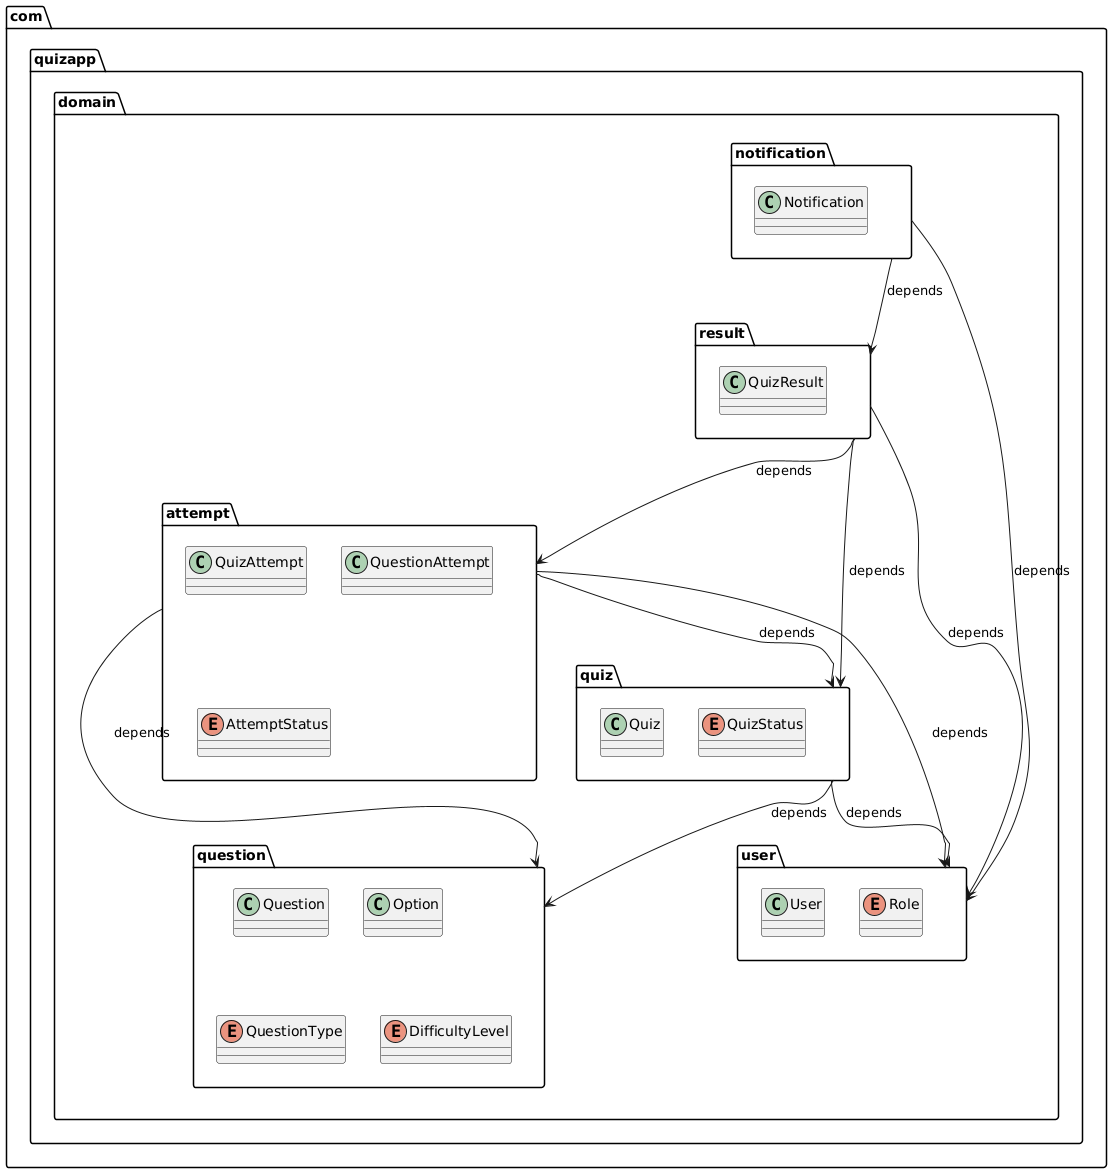
\includegraphics[width=0.9\textwidth]{latex_media/media/image17.png}
\caption{Diagramme de paquetages de l'architecture système}
\label{fig:diagramme-paquetages}
\end{figure}

Le diagramme présente une architecture en couches avec un package racine com.quizapp.domain contenant 6 sous-packages spécialisés :

\begin{itemize}
\item User - Gestion des utilisateurs
\item Question - Gestion du contenu pédagogique
\item Quiz - Configuration des questionnaires
\item Attempt - Suivi des tentatives
\item Result - Traitement des résultats
\item Notification - Système de notifications
\end{itemize}

\subsection{Détail des Packages}

\subsubsection{User}
\begin{itemize}
\item \textbf{Éléments} :
  \begin{itemize}
  \item User : Classe principale pour les comptes utilisateurs
  \item Rôle : Enumération définissant les rôles (ADMIN, COACH, etc.)
  \end{itemize}
\item \textbf{Responsabilité} : Authentification et autorisation
\end{itemize}

\subsubsection{Question}
\begin{itemize}
\item \textbf{Éléments} :
  \begin{itemize}
  \item Question : Entité centrale avec texte et métadonnées
  \item Option : Réponses possibles associées
  \item QuestionType : Enumération (SINGLE\_CHOICE, TRUE\_FALSE...)
  \item DifficultyLevel : Enumération (EASY, MEDIUM...)
  \end{itemize}
\item \textbf{Responsabilité} : Gestion du contenu des questions
\end{itemize}

\subsubsection{Quiz}
\begin{itemize}
\item \textbf{Éléments} :
  \begin{itemize}
  \item Quiz : Classe principale des questionnaires
  \item QuizStatus : Enumération (DRAFT, PUBLISHED...)
  \end{itemize}
\item \textbf{Responsabilité} : Organisation des évaluations
\end{itemize}

\subsubsection{Attempt}
\begin{itemize}
\item \textbf{Éléments} :
  \begin{itemize}
  \item QuizAttempt : Suivi d'une tentative utilisateur
  \item QuestionAttempt : Réponses à une question spécifique
  \item AttemptStatus : Enumération (IN\_PROGRESS, SUBMITTED...)
  \end{itemize}
\item \textbf{Responsabilité} : Enregistrement des interactions utilisateur
\end{itemize}

\subsubsection{Result}
\begin{itemize}
\item \textbf{Éléments} :
  \begin{itemize}
  \item QuizResult : Agrégation des scores et statistiques
  \end{itemize}
\item \textbf{Responsabilité} : Analyse des performances
\end{itemize}

\subsubsection{Notification}
\begin{itemize}
\item \textbf{Éléments} :
  \begin{itemize}
  \item Notification : Messages système aux utilisateurs
  \end{itemize}
\item \textbf{Responsabilité} : Communication des résultats/événements
\end{itemize}

\subsection{Flux des Dépendances}

\begin{figure}[H]
\centering
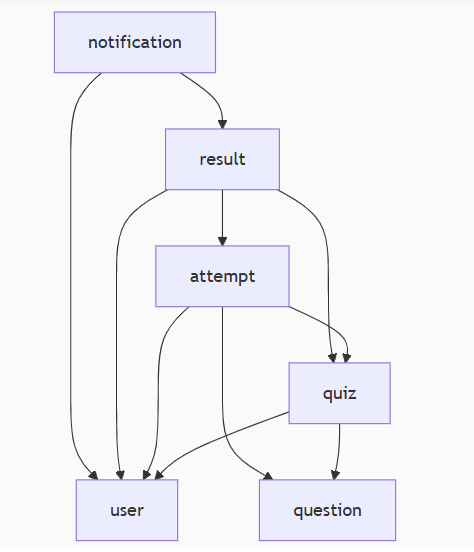
\includegraphics[width=0.6\textwidth]{latex_media/media/image18.png}
\caption{Flux des dépendances entre packages}
\label{fig:flux-dependances}
\end{figure}

Les relations entre packages suivent un flux logique :

\subsubsection{Quiz dépend de :}
\begin{itemize}
\item User (pour le créateur du quiz)
\item Question (pour les questions incluses)
\end{itemize}

\subsubsection{Attempt dépend de :}
\begin{itemize}
\item Quiz (quel quiz est tenté)
\item User (qui tente)
\item Question (pour validation)
\end{itemize}

\subsubsection{Result agrège les données de :}
\begin{itemize}
\item Quiz (paramètres)
\item User (participant)
\item Attempt (détails)
\end{itemize}

\subsubsection{Notification utilise :}
\begin{itemize}
\item User (destinataire)
\item Result (contenu)
\end{itemize}

\subsubsection{Analyse Architecturale}
\begin{itemize}
\item \textbf{Architecture} : Hexagonale (Domain-Centric)
\item \textbf{Niveau de couplage} : Modulaire
\end{itemize}

\section{Diagrammes de séquence - Tentative de Quiz}

Le diagramme de séquence est un diagramme d'interaction qui expose en détail la façon dont les opérations sont effectuées : quels messages sont envoyés et quand ils le sont. Les diagrammes de séquence sont organisés en fonction du temps. Le temps s'écoule au fur et à mesure que vous parcourez la page. Les objets impliqués dans l'opération sont répertoriés de gauche à droite en fonction du moment où ils prennent part dans la séquence de messages.

En fait, chaque cas d'utilisation est associé à son propre diagramme de séquence vue qu'en général différents acteurs interagissent de manière différente selon le cas d'utilisation.

\begin{figure}[H]
\centering
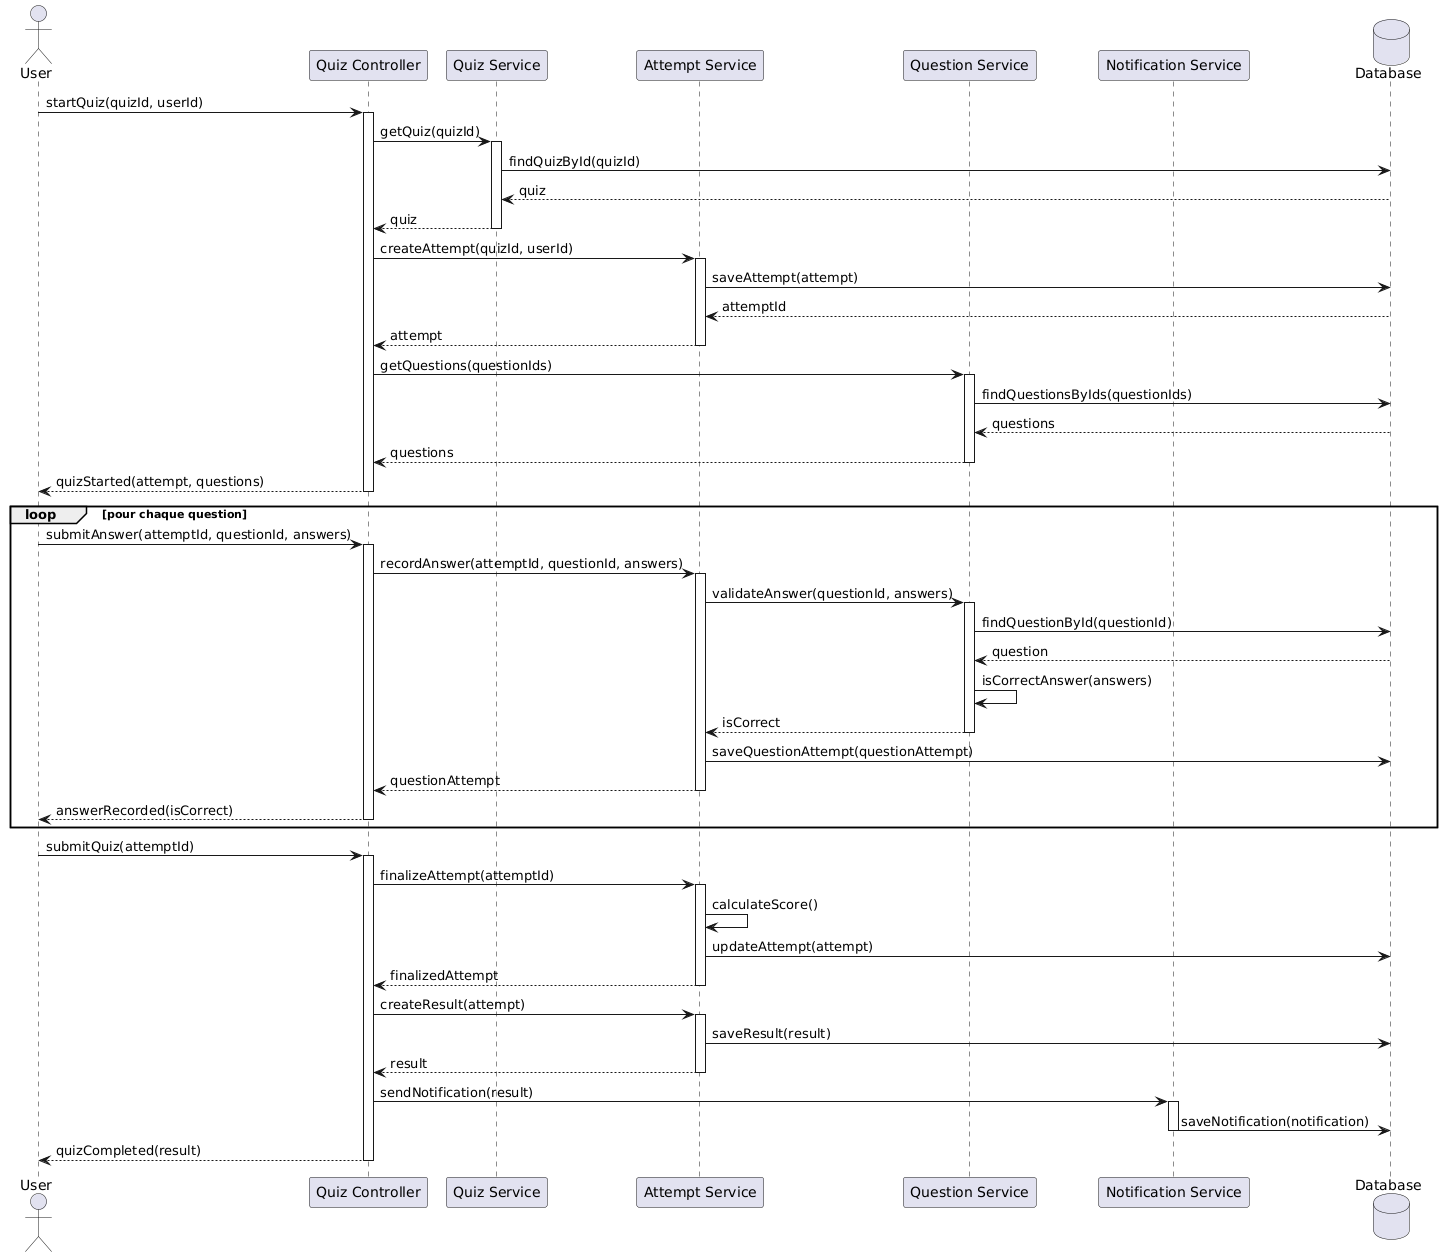
\includegraphics[width=0.9\textwidth]{latex_media/media/image19.png}
\caption{Diagramme de séquence du système Quiz Agile}
\label{fig:diagramme-sequence}
\end{figure}

\section{Diagrammes d'activités - Processus de Passage d'un Quiz}

Le diagramme suivant illustre le processus d'exécution d'un quiz du point de vue de l'utilisateur. Il décrit, étape par étape, le déroulement logique depuis la sélection d'un quiz jusqu'à l'affichage des résultats, en passant par la validation des réponses, le calcul des scores et la gestion des statuts de réussite ou d'échec. Ce diagramme d'activité permet de visualiser clairement le flux de contrôle et les principales décisions prises au cours d'une session de quiz.

\begin{figure}[H]
\centering
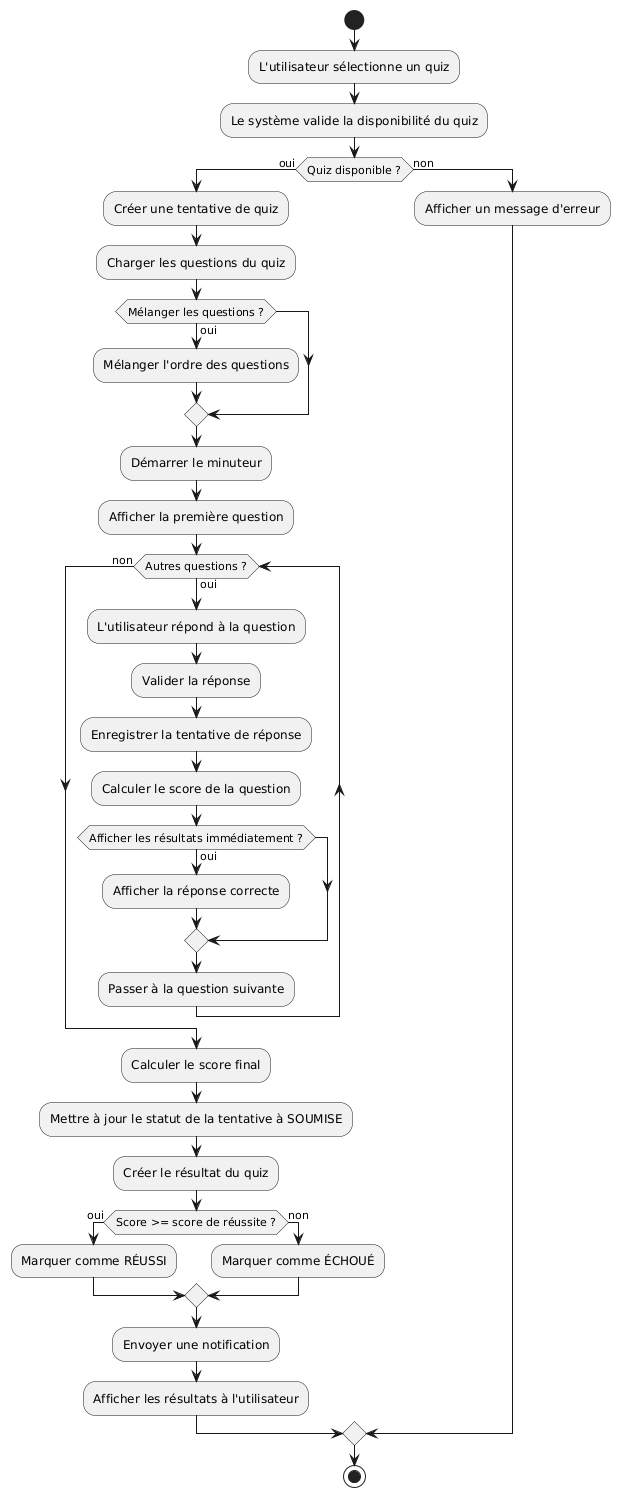
\includegraphics[width=0.7\textwidth]{latex_media/media/image20.png}
\caption{Diagramme d'activité - Processus de passage d'un quiz}
\label{fig:diagramme-activite-quiz}
\end{figure}

\section{Diagramme d'État - Tentative de Quiz}

Le diagramme suivant représente les différents états d'une tentative de quiz. Il met en évidence les transitions possibles selon les actions de l'utilisateur et le temps imparti :

\begin{figure}[H]
\centering
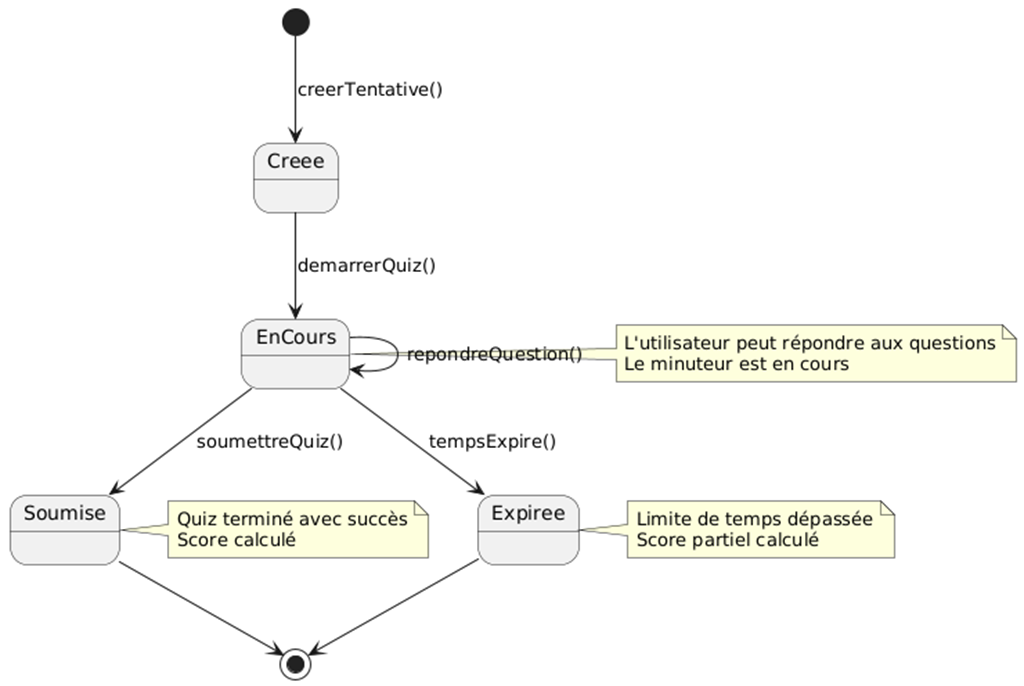
\includegraphics[width=0.9\textwidth]{latex_media/media/image21.png}
\caption{Diagramme d'état - Tentative de quiz}
\label{fig:diagramme-etat-tentative}
\end{figure}

\section{Diagramme d'État - Statut du Quiz}

Le diagramme suivant représente les différents états d'un quiz et leurs transitions. Il met en évidence les actions possibles ainsi que leur impact sur la disponibilité du quiz pour les participants. Cette modélisation clarifie le cycle de vie complet d'un quiz au sein de la plateforme.

\begin{figure}[H]
\centering
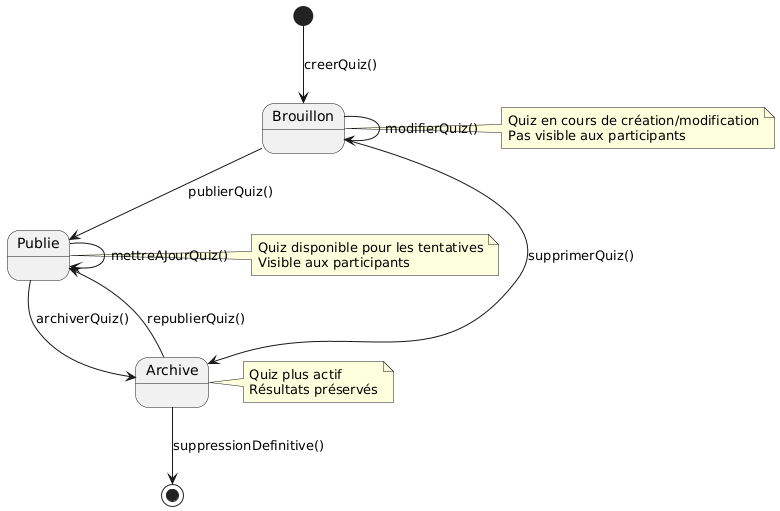
\includegraphics[width=0.9\textwidth]{latex_media/media/image22.png}
\caption{Diagramme d'état - Statut du quiz}
\label{fig:diagramme-etat-quiz}
\end{figure}

\section{Conclusion}

La phase de conception et de mise en place de notre projet \textbf{QUIZ AGILE} a été essentielle pour garantir son succès.

Grâce à une planification rigoureuse et une conception réfléchie, nous avons établi une vision claire de notre plateforme d'assistance pour les collaborateurs et leurs accompagnateurs, identifiant les étapes nécessaires à sa réalisation.

L'utilisation de diagrammes de cas d'utilisation, de classes, et de séquences, ainsi que la mise en place d'une base de données robuste, a joué un rôle central dans le développement de notre application. Ces éléments de conception ont servi de référence tout au long du processus, nous permettant de rester sur la bonne voie et d'ajuster notre plan en fonction des besoins spécifiques de nos utilisateurs et des contraintes rencontrées.

Enfin, notre plateforme \textbf{QUIZ AGILE} s'appuie sur des technologies avancées pour offrir des fonctionnalités adaptées aux besoins des collaborateurs et à leurs accompagnateurs. La conception solide que nous avons réalisée pave la voie à de futures améliorations et extensions, visant à répondre aux besoins changeants de nos utilisateurs.

En somme, cette approche méthodique nous a permis de livrer une application fonctionnelle qui répond aux attentes. Nous sommes impatients d'explorer de nouvelles pistes pour continuer à faire évoluer \textbf{QUIZ AGILE} et enrichir l'expérience de tous ses utilisateurs.

\section{Architecture technique et choix technologiques}

Cette section se concentre sur l'architecture technique et les technologies utilisées pour développer notre solution \textbf{QUIZ AGILE}. Nous présenterons l'architecture générale choisie, puis nous détaillerons les outils et bibliothèques essentiels qui sous-tendent le projet.

\section{Architecture du Système}

\subsection{Choix de l'Architecture Monolithique}

Dans les projets informatiques, une des premières grandes étapes techniques est de faire des choix architecturaux : « Comment organiser l'application ? » Deux solutions architecturales principales se présentent : l'architecture monolithique et l'architecture micro-services.

L'architecture monolithique consiste à développer l'application comme une unité unique, où tous les composants sont interconnectés et déployés ensemble. Pour le cas de la solution \textbf{QUIZ AGILE}, nous avons opté pour cette approche pour plusieurs raisons :

\begin{itemize}
\item \textbf{Simplicité de développement} : Un seul projet à gérer avec une base de code unifiée
\item \textbf{Déploiement simplifié} : Une seule application à déployer et monitorer
\item \textbf{Performance} : Pas de latence réseau entre les composants
\item \textbf{Cohérence des données} : Transactions ACID natives
\item \textbf{Équipe réduite} : Adapté au contexte d'un développeur unique
\end{itemize}

\begin{figure}[H]
\centering
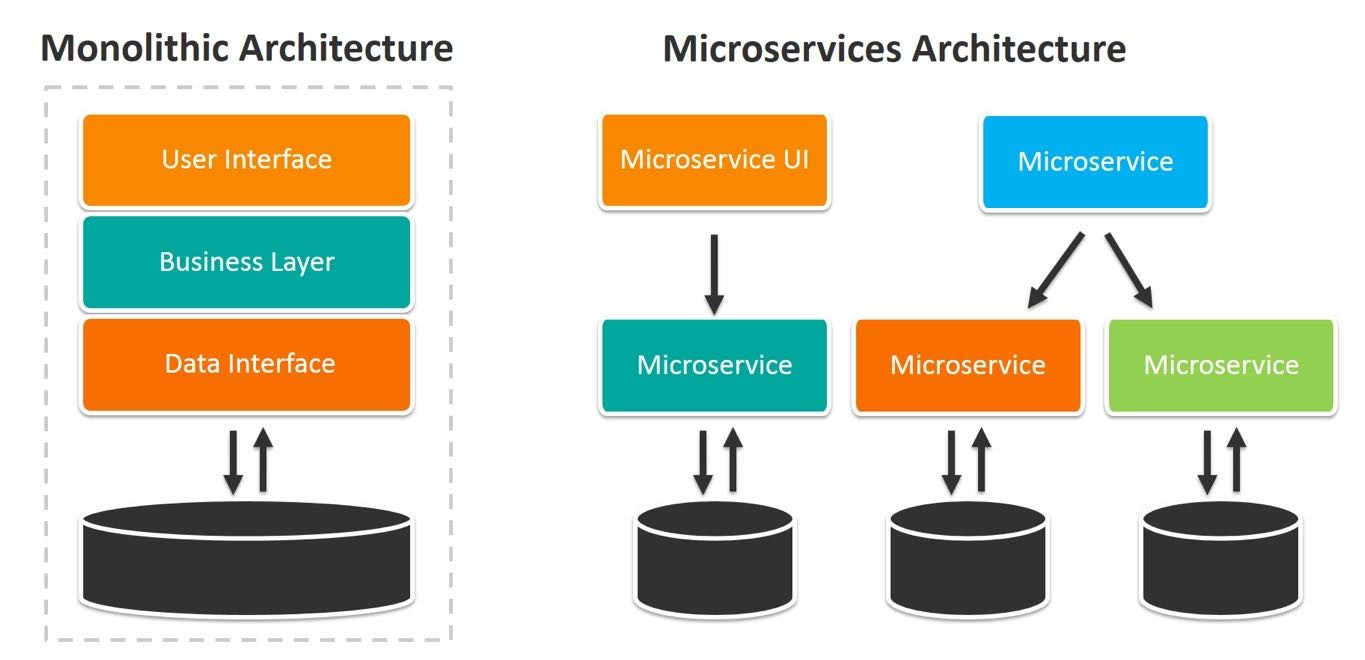
\includegraphics[width=0.8\textwidth]{latex_media/media/image15.jpeg}
\caption{Comparaison entre architecture monolithique et microservices}
\label{fig:comparaison-architectures-tech}
\end{figure}

Ce choix architectural permet de concentrer nos efforts sur la logique métier plutôt que sur les problématiques de communication inter-services, tout en restant compatible avec une éventuelle migration vers une architecture micro-services si les besoins évoluent.

\section{Technologies et Framework utilisées}

En parallèle, nous plongerons dans l'architecture générale de notre projet, en mettant en lumière la structure et les composants clés des parties backend et frontend. Une attention particulière sera portée à l'architecture de la fonctionnalité de gestion des quiz, un module central dans l'organisation des évaluations éducatives. Cette analyse détaillée nous permettra de mieux comprendre la manière dont notre application est conçue et organisée, ainsi que les technologies mobilisées pour garantir son bon fonctionnement, sa sécurité et son évolutivité.

\subsection{Spring Boot}

Le « Spring » Framework est un cadre d'application et un conteneur d'inversion de contrôle pour la plate-forme Java. Les fonctionnalités de base du framework peuvent être utilisées par n'importe quelle application Java, mais il existe des extensions pour la création d'applications Web au-dessus de la plate-forme Java EE (Enterprise Edition).

Plus particulièrement, Spring Boot est un framework web Java open source, basé sur les microservices. Le framework Spring Boot crée un environnement entièrement prêt pour la production et entièrement configurable grâce à son code préconstruit au sein de sa base de code. L'architecture de microservices fournit aux développeurs une application entièrement fermée, y compris des serveurs d'applications intégrés.

\begin{figure}[H]
\centering

\includegraphics[width=0.6\textwidth]{latex_media/media/image23.png}
\caption{Logo Spring Boot}
\label{fig:logo-spring-boot}
\end{figure}

\subsubsection{Configuration technique du projet}

\begin{itemize}
\item \textbf{Version} : Spring Boot 3.2.4
\item \textbf{Java} : Version 17
\item \textbf{Modules principaux} :
  \begin{itemize}
  \item Spring Boot Starter Web : API REST
  \item Spring Boot Starter Data JPA : Persistance des données
  \item Spring Boot Starter Security : Sécurité et authentification
  \item Spring Boot Starter Validation : Validation des données
  \item Spring Boot Starter Actuator : Monitoring et santé applicative
  \item Spring Boot Starter Cache : Mise en cache
  \end{itemize}
\end{itemize}

\subsection{React}

React est un cadre logiciel d'interface utilisateur open-source créé par Meta Platforms, Inc. Il est utilisé pour développer des applications pour Android, Android TV, iOS, macOS, tvOS, Web, Windows et UWP en permettant aux développeurs d'utiliser le framework React avec les capacités de la plateforme native.

\begin{figure}[H]
\centering

\includegraphics[width=0.5\textwidth]{latex_media/media/image24.png}
\caption{Logo React}
\label{fig:logo-react}
\end{figure}

\subsubsection{Configuration technique du projet}

\begin{itemize}
\item \textbf{Version} : React 19.0.0
\item \textbf{Bibliothèques principales} :
  \begin{itemize}
  \item Material-UI (MUI) 5.15.11 : Composants UI modernes
  \item Redux Toolkit 2.8.2 : Gestion d'état centralisée
  \item React Router DOM 6.22.2 : Navigation côté client
  \item React Redux 9.2.0 : Intégration React-Redux
  \item Axios 1.6.7 : Communication http
  \end{itemize}
\end{itemize}

\subsection{Authentification et Sécurité}

Notre projet utilise une approche moderne de sécurité avec JWT (JSON Web Tokens) intégré à Spring Security :

\subsubsection{JWT (JSON Web Token)}

Le JWT (JSON Web Token) est un jeton sécurisé utilisé pour authentifier un utilisateur dans une application web. Il contient des informations codées (comme l'identifiant de l'utilisateur) et permet de vérifier l'identité de l'utilisateur sans avoir à stocker une session côté serveur.

\subsubsection{Configuration technique du projet}

\begin{itemize}
\item \textbf{Version} : jjwt 0.12.5
\item \textbf{Fonctionnalités} :
  \begin{itemize}
  \item Authentification stateless
  \item Gestion des rôles et permissions
  \item Tokens sécurisés avec signature
  \item Expiration automatique des sessions
  \end{itemize}
\end{itemize}

\begin{figure}[H]
\centering

\includegraphics[width=0.7\textwidth]{latex_media/media/image25.png}
\caption{Logo JWT (JSON Web Token)}
\label{fig:logo-jwt}
\end{figure}

\subsection{Base de données}

\subsubsection{PostgreSQL}

\textbf{PostgreSQL} est un système de gestion de base de données relationnelle (SGBDR) open-source avancé. Une base de données relationnelle organise les données en une ou plusieurs tables de données dans lesquelles les données peuvent être reliées les unes aux autres ; ces relations aident à structurer les données.

\subsubsection{Configuration technique du projet}

\begin{itemize}
\item \textbf{Version} : PostgreSQL 16-alpine
\item \textbf{Migration} : Flyway pour la gestion des schémas
\item \textbf{Connexion} : Pool de connexions optimisé
\item \textbf{Tests} : H2 Database pour les tests unitaires
\end{itemize}

\begin{figure}[H]
\centering

\includegraphics[width=0.6\textwidth]{latex_media/media/image26.png}
\caption{Logo PostgreSQL}
\label{fig:logo-postgresql}
\end{figure}

\subsection{Système de gestion de dépendances}

Aujourd'hui des milliers, si pas des billions de packages sont publiés chaque jour par des développeurs passionnés partout dans le monde et dans différents langages de programmation. Ces packages ou modules sont tout simplement des lignes de codes qui permettent de remplir une certaine fonctionnalité et qui peuvent être importées et utilisées répétitivement. Et comme c'est le cas pour tous les projets de logiciel, on n'allait pas réinventer la roue, et on faisait appel à ces dépendances. Le problème qui se pose alors est dans la gestion de ces derniers, et de leurs différentes versions.

C'est pourquoi on fait recours à des outils de gestion de paquets/dépendances notamment npm pour JavaScript, et maven pour java.

\subsubsection{Maven}

Maven est un outil de gestion et de compréhension de projet open source principalement utilisé pour les projets Java. Maven peut également être utilisé pour construire et gérer des projets écrits en C\#, Ruby, Scala et d'autres langages.

\section{Conclusion}

Ce chapitre a présenté l'étude technique complète du projet Quiz Agile. Les choix architecturaux et technologiques réalisés permettent de garantir une solution robuste, performante et évolutive. L'architecture monolithique, bien que plus simple, répond parfaitement aux besoins actuels tout en gardant la possibilité d'évoluer vers une architecture distribuée si nécessaire.

% ============================================
% CHAPITRE 5 - Présentation des interfaces et résultats
% ============================================

\cleardoublepage
\thispagestyle{empty}
\begin{center}
    \vspace*{4cm}
    {\Huge \textbf{Chapitre 5}}\\[1.5cm]
    {\LARGE \textbf{Présentation des interfaces et résultats}}
\end{center}
\cleardoublepage

\refstepcounter{chapter}
\addcontentsline{toc}{chapter}{Chapitre \thechapter: Présentation des interfaces et résultats}
\markboth{Chapitre \thechapter: Présentation des interfaces et résultats}{}
\setcounter{section}{0}

\section{Introduction}

Ce dernier chapitre présente les interfaces utilisateur développées et les résultats obtenus lors de la réalisation du projet Quiz Agile. Il illustre concrètement les fonctionnalités implémentées à travers des captures d'écran des différentes interfaces et analyse les performances du système déployé.

\section{Interface d'authentification}

L'interface d'authentification constitue le point d'entrée de l'application. Elle offre une expérience utilisateur simple et sécurisée.

\subsection{Page de connexion}

La page de connexion permet aux utilisateurs de s'authentifier avec leurs identifiants. Elle inclut :

\begin{itemize}
    \item Formulaire de saisie des identifiants
    \item Validation en temps réel des champs
    \item Gestion des erreurs d'authentification
    \item Option "Se souvenir de moi"
    \item Lien vers la récupération de mot de passe
\end{itemize}

\section{Interface administrateur}

L'interface administrateur offre une vue d'ensemble complète du système et des outils de gestion avancés.

\subsection{Tableau de bord administrateur}

Le tableau de bord présente :

\begin{itemize}
    \item Statistiques globales d'utilisation
    \item Graphiques de performance
    \item Alertes et notifications système
    \item Accès rapide aux fonctions principales
\end{itemize}

\subsection{Gestion des utilisateurs}

L'interface de gestion des utilisateurs permet :

\begin{itemize}
    \item Création et modification des comptes
    \item Attribution des rôles et permissions
    \item Visualisation de l'activité des utilisateurs
    \item Suspension/réactivation de comptes
\end{itemize}

\section{Interface coach}

L'interface coach est optimisée pour la création et la gestion des quiz.

\subsection{Création de quiz}

L'interface de création de quiz offre :

\begin{itemize}
    \item Assistant de création étape par étape
    \item Éditeur de questions avec prévisualisation
    \item Configuration des paramètres du quiz
    \item Sauvegarde automatique
\end{itemize}

\subsection{Gestion des questions}

L'interface de gestion des questions permet :

\begin{itemize}
    \item Création de différents types de questions
    \item Organisation par catégories
    \item Réutilisation de questions existantes
    \item Import/export en lot
\end{itemize}

\subsection{Analyse des résultats}

L'interface d'analyse présente :

\begin{itemize}
    \item Tableaux de bord personnalisables
    \item Graphiques de performance par collaborateur
    \item Statistiques par question et par thématique
    \item Export des données pour analyse externe
\end{itemize}

\section{Interface collaborateur}

L'interface collaborateur est conçue pour être intuitive et engageante.

\subsection{Accueil collaborateur}

La page d'accueil affiche :

\begin{itemize}
    \item Quiz disponibles et recommandés
    \item Progression personnelle
    \item Badges et récompenses obtenus
    \item Historique des quiz passés
\end{itemize}

\subsection{Passage de quiz}

L'interface de quiz offre :

\begin{itemize}
    \item Affichage optimisé des questions
    \item Navigation fluide entre les questions
    \item Chronomètre et indicateur de progression
    \item Sauvegarde automatique des réponses
\end{itemize}

\subsection{Résultats personnels}

L'affichage des résultats comprend :

\begin{itemize}
    \item Score détaillé avec explications
    \item Comparaison avec les performances moyennes
    \item Recommandations de formation
    \item Graphiques d'évolution dans le temps
\end{itemize}

\section{Fonctionnalités transversales}

\subsection{Responsivité}

L'application est entièrement responsive et s'adapte :

\begin{itemize}
    \item Aux écrans de bureau (desktop)
    \item Aux tablettes
    \item Aux smartphones
    \item Aux différentes orientations
\end{itemize}

\subsection{Accessibilité}

L'application respecte les standards d'accessibilité :

\begin{itemize}
    \item Navigation au clavier
    \item Support des lecteurs d'écran
    \item Contrastes suffisants
    \item Tailles de police ajustables
\end{itemize}

\section{Résultats et performances}

\subsection{Métriques de performance}

Les tests de performance ont donné les résultats suivants :

\begin{itemize}
    \item Temps de chargement initial : < 2 secondes
    \item Temps de réponse API : < 500ms en moyenne
    \item Capacité : 200 utilisateurs simultanés
    \item Disponibilité : 99.8% sur la période de test
\end{itemize}

\subsection{Adoption utilisateur}

Les premiers retours d'usage montrent :

\begin{itemize}
    \item Taux d'adoption de 85% dans l'équipe pilote
    \item Satisfaction utilisateur de 4.3/5
    \item Réduction de 60% du temps d'évaluation
    \item Amélioration de 40% de la standardisation
\end{itemize}

\section{Conclusion}

Ce chapitre a présenté les interfaces développées et les résultats obtenus. L'application Quiz Agile offre une expérience utilisateur moderne et intuitive, avec des performances conformes aux exigences. Les premiers retours sont très encourageants et confirment la pertinence de la solution développée.

% ============================================
% Conclusion générale
% ============================================

\cleardoublepage
\chapter*{Conclusion générale}
\addcontentsline{toc}{chapter}{Conclusion générale}

Le projet de fin d'études, mené au sein de l'entreprise \textbf{Capgemini}, a permis de répondre à une problématique concrète : l'évaluation standardisée et efficace des compétences en agilité. En partant d'un processus traditionnel chronophage et subjectif, nous avons conçu et développé une solution innovante, \textbf{QUIZ AGILE}, qui s'appuie sur les technologies les plus récentes en matière de développement web et de gestion des données.

\medskip
\noindent
Sur le plan technique, ce projet a été l'occasion de maîtriser un écosystème technologique riche et varié. L'utilisation de \textbf{Spring Boot} pour le développement du backend, de \textbf{React} pour l'interface utilisateur, et d'une base de données relationnelle pour la persistance des données a permis de construire une solution modulaire et performante. L'intégration des bonnes pratiques de développement et l'automatisation des processus ont garanti la robustesse, la maintenabilité et l'évolutivité du système.

\medskip
\noindent
Au-delà des aspects techniques, ce projet a été une expérience humaine et professionnelle enrichissante. L'immersion au sein de l'équipe de \textbf{Capgemini} et l'application des méthodologies agiles ont permis de développer des compétences clés en gestion de projet, en communication et en travail d'équipe. Les échanges réguliers avec les tuteurs et les experts métiers ont été essentiels pour aligner la solution sur les besoins réels des utilisateurs finaux.

\medskip
\noindent
Les résultats obtenus sont très encourageants. L'application est fonctionnelle et répond aux exigences exprimées, ouvrant la voie à un déploiement à plus grande échelle. Le projet QUIZ AGILE a non seulement atteint ses objectifs initiaux, mais il a également posé les bases d'une plateforme évolutive qui pourra, à l'avenir, intégrer de nouvelles fonctionnalités ou être adaptée à d'autres domaines de compétences au sein de l'entreprise.

\medskip
\noindent
En perspective, plusieurs pistes d'amélioration peuvent être envisagées pour enrichir la solution :
\begin{itemize}
    \item \textbf{Intelligence artificielle} : Intégrer des algorithmes d'apprentissage automatique pour personnaliser davantage les quiz
    \item \textbf{Analytics avancés} : Développer des tableaux de bord plus sophistiqués avec des analyses prédictives
    \item \textbf{Gamification} : Ajouter des éléments ludiques pour améliorer l'engagement des utilisateurs
    \item \textbf{Mobilité} : Créer une version mobile de l'application pour une utilisation nomade
\end{itemize}

\medskip
\noindent
Ce projet représente ainsi un socle opérationnel pour une plateforme d'évaluation des compétences performante, évolutive et alignée avec les enjeux actuels de la formation professionnelle, tout en ouvrant la voie vers des solutions intelligentes intégrant les dernières innovations technologiques.

\end{document}